
\documentclass[11pt, a4paper]{book}
\usepackage{svn-multi}
\svnid{$Id$}
\usepackage{prelim2e}
\renewcommand{\PrelimWords}{\svnkw{Id}}
%%\newcommand*{\mysvnrev}{\svnrev}
\usepackage[hyperindex=true,
			bookmarks=true,
            pdftitle={}, pdfauthor={Xi Yang},
            colorlinks=false,
            pdfborder=0,
            pagebackref=false,
            citecolor=blue,
            plainpages=false,
            pdfpagelabels,
            pagebackref=true,
            hyperfootnotes=false]{hyperref}
\usepackage[all]{hypcap}
\usepackage[palatino, draft]{anuthesis}
\usepackage{afterpage}
\usepackage{graphicx}
\usepackage{caption}
\usepackage{thesis}
\usepackage{amsmath}
\usepackage{bm}
\usepackage{amsthm}
\usepackage{subcaption}
\usepackage{algorithm}
\usepackage{algpseudocode}
\usepackage{amssymb}
\usepackage[round, authoryear]{natbib}
\usepackage[normalem]{ulem}
\usepackage[table]{xcolor}
\usepackage{makeidx}
\usepackage{cleveref}
\usepackage{caption}
\usepackage{float}
\urlstyle{sf}
\renewcommand{\sfdefault}{uop}
\usepackage[T1]{fontenc}
\usepackage[scaled]{beramono}

\usepackage{multirow}

\theoremstyle{definition}
\newtheorem{theorem}{Theorem}
\newtheorem{definition}{Definition}
\newtheorem{example}{Example}
\newtheorem{remark}{Remark}
\newtheorem{lemma}{Lemma}
\newtheorem{proposition}{Proposition}
\newtheorem{condition}{Condition}
\newtheorem{assumption}{Assumption}

\renewcommand*{\backref}[1]{}
\renewcommand*{\backrefalt}[4]{
  \ifcase #1 %
    %
  \or
    (cited on page #2)%
  \else
    (cited on pages #2)%
  \fi
}




\input{macros}            
%%%%%%%%%%%%%%%%%%%%%%%%%%%%%%%%%%%%%%%%%%%%%%%%%%%%%%%%%%%%%%%%%%%%%%%
%% Preamble
\title{Factor Analytic Distributed Multinomial Model}
\author{Mingyang Sheng}
\date{\today}

\renewcommand{\thepage}{\roman{page}}

\makeindex
\begin{document}
%\doparttoc
%%%%%%%%%%%%%%%%%%%%%%%%%%%%%%%%%%%%%%%%%%%%%%%%%%%%%%%%%%%%%%%%%%%%%%%
%% Title page
\pagestyle{empty}
\thispagestyle{empty}
\input{titlepage}

%%%%%%%%%%%%%%%%%%%%%%%%%%%%%%%%%%%%%%%%%%%%%%%%%%%%%%%%%%%%%%%%%%%%%%%
%% Here begin the preliminaries
\input{frontmatter}

%%%%%%%%%%%%%%%%%%%%%%%%%%%%%%%%%%%%%%%%%%%%%%%%%%%%%%%%%%%%%%%%%%%%%%%
%% Dedication
\cleardoublepage
\pagestyle{empty}
\input{dedication}

%%%%%%%%%%%%%%%%%%%%%%%%%%%%%%%%%%%%%%%%%%%%%%%%%%%%%%%%%%%%%%%%%%%%%%%
%% Acknowledgements
\cleardoublepage
\pagestyle{empty}
\input{ack}

%%%%%%%%%%%%%%%%%%%%%%%%%%%%%%%%%%%%%%%%%%%%%%%%%%%%%%%%%%%%%%%%%%%%%%%
%% Abstract
\cleardoublepage
\pagestyle{headings}
\input{abstract}

%%%%%%%%%%%%%%%%%%%%%%%%%%%%%%%%%%%%%%%%%%%%%%%%%%%%%%%%%%%%%%%%%%%%%%%
%% Table of contents
\cleardoublepage
\pagestyle{headings}
\markboth{Contents}{Contents}
\tableofcontents
\listoffigures
\listoftables


%%%%%%%%%%%%%%%%%%%%%%%%%%%%%%%%%%%%%%%%%%%%%%%%%%%%%%%%%%%%%%%%%%%%%%
%% Here begins the main text
\mainmatter

%% Introduction
\chapter{Introduction}
\label{cha:intro}

% Multinomial data naturally arise in many applications where observations are distributed across a finite set of mutually exclusive categories. For example, in market research, the number of consumers choosing among several (competing) brands [CITATION]; in public health studies, the number of individuals falling into different health status categories [CITATION]; and in text analysis, the word count from a fixed vocabulary from sampled books [CITATION]. These multinomial counts are, however, often associated with covariates or grouping structures whose relationships with the observed counts are of substantive interest.

% Multinomial, common questions
Multinomial data arise naturally in many applications. Observations are distributed across a finite set of mutually exclusive categories. For example, \citet{zhang2026conjugatingvariationalinferencelarge} used mixed multinomial logit model to analyse the number of consumers choosing among several competing brands in market research. In public health, \citet{Beltran2024} models the number of individuals falling into different health status categories. In text analysis, word counts from a fixed vocabulary are used to characterise sampled documents \citep{Taddy_2015}. These multinomial counts rarely arise in isolation. They are typically associated with covariates describing the observations and group structure. The relationship between this structure and the observed counts is of substantive interest.

% Example, previous work: multinomial(pme, dmr) -> reduced-rank structutre 
A large body of previous work models the category probabilities as a function of covariates and group membership. The multinomial logistic regression model is the classical starting point. It extends naturally to a mixed-effects model that adds a group-level random effect to capture within-group correlation, which is an approach that still under active development at large scale for multinomial choice data with many groups \citep{zhang2026conjugatingvariationalinferencelarge}. In recent years, there has been a growing movement towards the application of high-dimensional multinomial datasets with large number of categories and groups. Previous work on large number of groups has been structured both theoretically and practically [Citation].

% Limitations in high-dim cases -> our work (fa-dmr)
However, the large-Q regimes are not discussed in the common work, which have arisen in many applications. As mentioned before, vocabulary sizes in text analysis are typically in the thousands \citep{Taddy_2015}. Taxon or gene counts in bioinformatics and genomics can run into the thousands. Spatial count data are often recorded over large numbers of small areal units \citep{Banerjee2008}. Due to the coupled nature of the multinomial distribution, computing the probability of a particular category requires considering the probabilities of all categories. This coupling not only increases the computationally cost as the number of categories grows, but also prevents the likelihood from being naturally decomposed across categories, posing challenges for scalable computation and inference. In the meanwhile, this bottleneck happens when we introduce the group structure $\bm{\lambda}$ into multinomial distribution, since the covariance $\operatorname{Cov}\left(\bm{\lambda}\right)$ has $\mathcal{O}(Q^2)$ free parameters. This is far more than any realistic number of groups $J$ can identify. It also means the $Q \times Q$ matrix operations that any likelihood-based procedure needs, such as inversion or computing a determinant, cost $O(Q^3)$, regardless of identifiability. Previous work faces obstructs on algorithms as well. \citet{Goplerud_2024} showed that standard mean-field coordinate ascent variational inference (CAVI) systematically under-estimates posterior uncertainty in high-dimensional mixed models with the degree of under-estimation worsening as dimension grows. \citet{Henderson02102019} faced similar difficulty for the alternative approach of maximum likelihood estimation via the EM algorithm, whose convergence rate is linear. This is a serious practical bottleneck for high-dimensional scenarios. 

The multinomial likelihood's row-total constraint $\sum_q \pi_{ijq}=1$ couples its categories together. This makes the observed-data Hessian dense and expensive to invert as $Q$ grows. 

% factor analyzer
A key approach for solving this obstruct is reduced-rank method. Multivariate random effects can be represented parsimoniously using a reduced-rank approach, which makes simplifying assumptions that reduce the dimension of the problem to $K\ll Q$ and fit a multivariate random effect via a linear combination of $K$ latent variables \citep{Bartholomew2011}. This framework is often referred to as a factor analytical model \citep{Bartholomew2011}, which has been used frequently in ecology and the social sciences. In the case of exponential family responses, it is sometimes called a generalized latent variable model (GLVM) \citep{Anders2004}.(check)
is not simply a matter of scale. Left unstructured, the group-level covariance $\Sigma = \mathrm{Cov}(\bm{\lambda})$ has $O(Q^2)$ free parameters. This is far more than any realistic number of groups $J$ can identify. It also means the $Q \times Q$ matrix operations that any likelihood-based procedure needs, such as inversion or computing a determinant, cost $O(Q^3)$, regardless of identifiability. Two broad families of estimation strategy are used to fit models of this kind. The first treats the group-level random effects $\bm{\lambda}_j$ as missing data, to be integrated out of the likelihood. This integration is done exactly where feasible, or via a Laplace approximation to the resulting intractable integral, within an EM algorithm that alternates between this approximate integration step and updating the remaining parameters. The second treats the same integration problem variationally, replacing the true posterior of $\bm{\lambda}$ with a tractable approximating family, most commonly a mean-field Gaussian fit by coordinate ascent (CAVI).

For multinomial distribution, many approaches are established to simplify the statistical modelling. \citet{Baker1994} exploited the Poisson-Multinomail Equivalence (PME) to decouple the multinomial likelihood as the product of independent-Poisson likelihood conditional on the individual total. \citet{Taddy_2015} adopted this work and established Distributed Multinomial Regression (DMR), which reduced a coupled $Q$-category regression to $Q$ independent Poisson regressions and applied on high-dimensional dataset.  
 
\todo{Describe what models are used to analyse this like below}

A natural approach to make inferences between covariates, cluster groups and the multionmial counts is to use a modelling approach. For $i = 1, 2, \dots, I$ in $j = 1, 2, ..., J$ and $q = 1, 2, ..., Q$, suppose that 

\begin{itemize}
\item  $y_{ijq}$ is the count in category $q$ for the $i$-th observation in cluster group $j$,
\item $\boldsymbol{y}_{ij} = (y_{ij1}, y_{ij2}, \cdots, y_{ijQ})^\top \in \mathbb{Z}^{Q}_{\geq 0}$ is the $Q\times 1$ vector of counts for the $i$-th observation and $j$-th group, and 
\item $x_{ijk}$ is the $k$-th covariate for the $i$-th observation in the $j$-th group.
\end{itemize}

\noindent Then we model ....

\todo{Introduce the problem when $Q$ is large}

with a massive number of categories have been used extensively in text analysis \citep{Taddy_2015}, bioinformatics \citep{Smith2001, Buettner2015} (socail science, economic) and spatial statistics \citep{Cressie2008, Banerjee2008}. 


\todo{Then describe the parameter estimation methods}

 A natural way to resolve this tension between flexibility and tractability is to impose a reduced-rank, factor-analytic structure directly on group-level random effect $\bm{\lambda}$. This avoids estimating an unstructured $\Sigma$ and then correcting for the resulting instability. Write $\alpha_j = B f_j + \varepsilon_j$, for a $Q \times K$ loading matrix $B$ with $K \ll Q$, a $K$-dimensional latent factor score $f_j$, and idiosyncratic noise $\varepsilon_j \sim \mathcal{N}(0, \sigma^2 I_Q)$. This reduces the number of free covariance parameters from $O(Q^2)$ to $O(QK)$ \citep{Bartholomew2011}. This construction is the classical factor-analytic model \citep{AndersonRubin1956,Bartholomew2011}, long used in ecology and the social sciences. It is sometimes called a generalised latent variable model (GLVM) when the observed responses follow an exponential-family distribution \citep{Anders2004}\todo{verify this GLVM attribution before submission}. A related, parallel line of work reaches for the same reduced-rank idea from a log-normal-Poisson rather than a multinomial starting point \citep{Batardiere2024}. We discuss the relationship between the two traditions in Chapter~\ref{cha:model-specification}.
 
In this thesis, we start from data that follow the multinomial distribution directly, which is the natural distribution for count data rather than one instance of a general exponential-family response. We denote latent factors $\mathbf{f}$ as missing data and $\bm{\lambda}$ as group-level random effects and imposes the factor-analytic and reduced-rank structure discussed above on the decomposition $\bm{\lambda}=\mathbf{B}\mathbf{B}^{\top}+\mathbf{D}$, then use an Expectation-Maximization (EM) algorithm to handle the resulting incomplete-data problem with unobserved $\mathbf{f}$ . Using the Poisson-multinomial equivalence introduced above \citep{Baker1994, Taddy_2015, lee2017poissontrickextensionsfitting}, we decouple thecomputation of Hessian. This accelerates each EM iteration from cubic to near-linear cost in $Q$. We further establish conditions under which the resulting estimator is consistent and asymptotically normal. These conditions are expressed in terms of the joint growth of the number of groups $J$ and the number of categories $Q$, rather than in terms of $Q$ alone. Recent work has pursued a related reduced-rank idea for item-level count data via joint maximum likelihood \citep{Cui2026} instead of EM algorithm. They discussed EM algorithm and its statistical properties as an open problem since the marginal likelihood maximization suffers more difficulties when dealing with integration of latent factors. As well,  we extend their model structure particularly in allowing genuine idiosyncratic variance to be considered, rather than the reduced-rank structure only. 
 
The remainder of the thesis is organised as follows. Chapter~\ref{cha:model-specification} introduces the model in full with identifiability conditions. It reviews the high-dimensional multivariate count factor-analytic literature and its extensions, and introduces the PME and the classical EM algorithm formally. Chapter~\ref{cha:methodology} develops the dense EM algorithm and the PME\&Woodbury-accelerated version. It discusses convergence and sources of approximation error, and compares the computational cost of our approach with the methods surveyed above. Chapter~\ref{cha:simulation-result} reports simulation studies. Chapter~\ref{cha:real-result} applies the model to real grouped count data. Chapter~\ref{cha:conc} concludes, discussing limitations and directions for future work. Commonly used notation is summarized in Table~\ref{tab:notation}.

\iffalse
In this thesis, we start with data that follows the Multinomial distribution, which is always used in counting dataset, instead of starting with the exponential family. Focus on reduced-rank structure in factor-analytic model, we use Expectation-Maximization (EM) Algorithm to deal with incomplete data with unknown latent variables. Given the Poisson-Multinomial Equivalence (PME) \citep{10.2307/2348134, lee2017poissontrickextensionsfitting}, we decouple the structure of Multinomial Hessian matrix and accelerate the EM algorithms with latent variables. 

In the next Chapter, we provide our model setup with identifiability conditions, an overview of the (high-dimensional) multivariate count factor-analytic models and extensions, the introduction of PME, and the brief introduction of classical EM algorithm. In Chapter~\ref{cha:methodology}, we describe the dense EM algorithm and Woodbury acceleration method decoupling by PME auxiliary variable structure. We discuss its convergence and sources of error. Furthermore, we compare the performance and computational efficiency of our proposed model with those of competing models reported in the literature review. Simulation studies and real data analysis are given in Chapter~\ref{cha:simulation-result} and \ref{cha:real-result}. Chapter~\ref{cha:conc} concludes the thesis, giving the limitation and future work.  

This thesis is organised as follows. The notation commonly used is summarised in Table~\ref{tab:notation}. Chapter~\ref{cha:model-specification} describes the background,  Chapter~\ref{cha:methodology} describes the main methodology in this thesis, Chapter~\ref{cha:simulation-result} shows the simulation result, Chapter~\ref{} demonstrates a real data application and we end with Chapter.
\fi

\newpage
\begin{table}[H]
\centering
\begin{tabular}{cc}
\hline
\textbf{Notation}    & \textbf{Definition or Description}               \\ \hline
$i$                    & Observation Index $i=1,2,\dots,I$           \\
$j$                    & Group Index $j=1,2,\dots,J$                 \\
$q$                    & Category Index $q=1,2,\dots,Q$              \\
$k$                    & Latent Index $k=1,2,\dots,K$                \\
$\bm{y}_{ij}$                     & The $i$-th observation in $j$-th group                                                 \\
$y_{ij\cdot}$                     & Observation Total Sum                                                 \\
PME                     & Poisson-Multinomial Equivalence (introduced in~\ref{sec:PME})                                                 \\
$\mathbf{B}$                    & Loading Matrix in $\mathbf{R}^{Q\times K}$       \\
$\mathbf{D}$                    & Idiosyncratic Matrix in $\mathbf{R}^{Q\times Q}$ \\
$\mathbf{f}$                     & Latent Vector                                                 \\
                     &                                                  \\
\multicolumn{1}{l}{} & \multicolumn{1}{l}{}                             \\
\multicolumn{1}{l}{} & \multicolumn{1}{l}{}                             \\
\multicolumn{1}{l}{} & \multicolumn{1}{l}{}                             \\ \hline
\end{tabular}
\end{table}
%% Chapters
\chapter{Background}
\label{cha:model-specification}

This chapter has three parts. Section~\ref{sec:model-setup-assumption} sets out the model, the Poisson--Multinomial equivalence, and the identifiability constraints the model requires. Section~\ref{sec:literature-review} reviews the related literature. Section~\ref{sec: em-algorithm-relatives} reviews the classical EM algorithm and the methods most closely related to ours.
% REVISION NOTE: the original roadmap paragraph referenced \ref{sec:model-setup} and \ref{sec:PME}, neither of which matched an existing \label in this chapter (the section is actually labelled sec:model-setup-assumption, and no \label{sec:PME} existed anywhere). The stated order (model setup, literature review, PME, EM) also did not match the chapter's actual order (model setup+PME together, then literature review, then EM). I added \label{sec:PME} at the natural point below (just before the Baker1994 discussion) and rewrote this paragraph to match the real structure. Please grep the rest of the thesis for \ref{sec:model-setup} and \ref{sec:PME} in case the old broken references are used elsewhere too.

\section{Models \& Assumptions}
\label{sec:model-setup-assumption}

\subsection{Model Setup}
\label{subsec:model-setup}

Let $\bm{y}_{ij}=(y_{ij1},\dots,y_{ijQ})^\top\in\mathbb{Z}_{\geq0}^Q$ be the response for observational unit $i=1,2,\dots,I_j$ in group $j=1,2,\dots,J$. The entries of $\bm{y}_{ij}$ are counts over $Q$ distinct categories. A vector of covariates $\bm{v}_{ij}\in\mathbb{R}^P$ is also recorded for each unit. Let $y_{ij\cdot}=\sum_{q=1}^Q y_{ijq}$ denote the multinomial total for unit $i$ in group $j(i)$. We omit a constant term from $\bm{v}_{ij}$, since it would be redundant with the category-specific intercepts already captured by $\bm\mu$. Conditional on the total count $y_{ij\cdot}$ and on the random effect $\bm\lambda_j\in\mathbb{R}^Q$, each observation follows a multinomial distribution,
\begin{equation}
\bm{y}_{ij}\mid y_{ij\cdot},\bm\lambda_j\sim\operatorname{Multinomial}\left(y_{ij\cdot},\,\bm{p}_{ij}\right),\qquad p_{ijq}=\frac{\exp(\eta_{ijq})}{\sum_{q'=1}^Q\exp(\eta_{ijq'})},
\label{eq:conditional-pm}
\end{equation}
with log-linear predictor
\begin{equation}
\eta_{ijq}=\mu_q+\bm{v}_{ij}^\top\bm\phi_q+\lambda_{jq},\qquad q=1,2,\dots,Q,
\label{eq:linear-predictor}
\end{equation}
where $\mu_q\in\mathbb{R}$ is the category-specific intercept and $\bm\Phi=(\bm\phi_1,\dots,\bm\phi_Q)$ collects the category-specific coefficient vectors.
% REVISION NOTE: added a definition for \bm\Phi. The symbol was used later, in "(\bm\mu,\bm\Phi,\bm\lambda_j)", without ever being introduced; please confirm this is the intended definition.
This thesis is concerned with the contribution $\bm\lambda_j$ of group $j$ to the log-relative-rate of category $q$. Equation~\eqref{eq:linear-predictor} extends the linear predictor of DMR \citep{Taddy2015} and of the Poisson extension of \citet{Lee2017}; the three models differ only in the distribution placed on $\bm\lambda_j$.

% The softmax link in Equation~\eqref{eq:conditional-pm} is invariant under the shift $\eta_{ijq}\mapsto\eta_{ijq}+c_{ij}$ for any constant $c_{ij}$ common to all categories, so the intercepts $\bm\mu=(\mu_1,\dots,\mu_Q)$ are identified only up to an additive constant. We remove this indeterminacy with the constraint $\sum_q\mu_q=0$.

% REVISION NOTE: the original sentence continued "...which automatically restores by the Poisson representation introduced below." I could not work out what this clause was asserting (restores what, exactly?) and have removed it rather than guess. If you meant that the sum-to-zero constraint on mu is mirrored by an analogous constraint that falls out of the Poisson representation below, please restate that explicitly and I will fold it back in precisely.

Throughout, we treat the total $y_{ij\cdot}$ as ancillary for $(\bm\mu,\bm\Phi,\bm\lambda_j)$. We assume its distribution carries no information about these parameters beyond what is already encoded in $\bm{p}_{ij}$, so conditioning on $y_{ij\cdot}$ in Equation~\eqref{eq:conditional-pm} loses no relevant information. This is standard practice in multinomial regression, but it is an assumption, not an automatic consequence of the model, and we do not attempt to model volume and composition jointly here. To be precise, ancillarity is a statement about information, not about determinism: the total is still random, and only its distribution is assumed uninformative about $(\bm\mu,\bm\Phi,\bm\lambda_j)$. Later in this section we use the Poisson-Multinomial equivalence to represent each $y_{ijq}$ as an independent Poisson variate whose offset $\xi_{ij}$ absorbs the random total; conditioning on $y_{ij\cdot}$ recovers Equation~\eqref{eq:conditional-pm} exactly. We treat $\xi_{ij}$ as a computational device, not as a modeling claim about the total.

The group random effects are assumed independently and identically distributed,
\begin{equation}
\bm\lambda_j\sim\mathcal{N}(\bm0,\bm\Sigma),\qquad\bm\Sigma=\mathbf{B}\mathbf{B}^\top+\mathbf{D},
\label{eq: Overall notation structure}
\end{equation}
where $\mathbf{B}\in\mathbb{R}^{Q\times K}$ is the factor-loading matrix and $\mathbf{D}$ is the idiosyncratic-variance matrix. Equivalently, in factor-regression form,
\begin{equation}
\bm\lambda_j=\mathbf{B}\mathbf{f}_j+\bm\epsilon_j,\qquad\mathbf{f}_j\sim\mathcal{N}(\bm0,\mathbf{I}_K),\qquad\bm\epsilon_j\sim\mathcal{N}(\bm0,\mathbf{D}),
\label{eq: Detailed notation structure}
\end{equation}
so that $\lambda_{jq}=\mathbf{b}_q^\top\mathbf{f}_j+\epsilon_{jq}$, where $\mathbf{b}_q$ is the $q$-th row of $\mathbf{B}$. Each group $j$ has a $K$-dimensional factor $\mathbf{f}_j$, where $K$ is known and $K<Q$. In this application, each entry of a loading row $\mathbf{b}_q$ measures how strongly category $q$ loads on a given latent factor, so $\mathbf{f}_j$ summarizes cluster-level information shared across categories. We follow \citet{Cui2026} in assuming the $K$ latent factors are mutually independent, as in Equation~\eqref{eq: Detailed notation structure}. Finally, for model simplicity we assume $\mathbf{D}=\sigma^2\mathbf{I}_Q$ with $\sigma^2>0$, rather than the fully diagonal $\mathbf{D}=\operatorname{diag}(d_1^2,\dots,d_Q^2)$ with $d_q>0$.
% Revison: change the reason of choosing isotropic variance

\paragraph{Poisson-Multinomial equivalence.}
\label{sec:PME}
The Poisson-Multinomial equivalence established by \citet{Baker1994} states that the multinomial likelihood conditional on the individual sum $y_{ij\cdot}$ is exactly equivalent to a product of independent Poisson likelihoods sharing a common additive offset,
\begin{equation}
\xi_{ij}=\log y_{ij\cdot}-\log\sum_{q=1}^Q\exp(\eta_{ijq}).
\label{eq:xi_baker}
\end{equation}
The joint draw $\bm{y}_{ij}\mid\bm\lambda_j\sim\operatorname{Multinomial}(y_{ij\cdot},\bm{p}_{ij})$ is equivalent to $y_{ijq}\mid\bm\lambda_j\sim\operatorname{Poisson}(\exp(\eta_{ijq}+\xi_{ij}))$ independently across $q=1,\dots,Q$, conditional on $y_{ij\cdot}$, with $\eta_{ijq}$ and $\bm{p}_{ij}$ as defined in Equations~\eqref{eq:conditional-pm}--\eqref{eq:linear-predictor}. The offset in Equation~\eqref{eq:xi_baker} absorbs the softmax normalizer and decouples the $Q$ Poisson problems, so they can be solved independently.

\citet{Lee2017} extended the framework of \citet{Baker1994} by treating the aggregate count $y_{ij\cdot}$ itself as Poisson-distributed given the group effect $\bm\lambda_j$, rather than fixing it as the conditioning variable in the multinomial likelihood. Marginalizing over this random aggregate recovers the same factorization into independent Poisson components across $q=1,\dots,Q$; $\xi_{ij}$ then becomes the rate parameter of the induced Poisson distribution rather than a fixed conditioning quantity. In our EM algorithm, the M-step therefore can be decomposed into $Q$ parallel GLM problems, one per category.

Our model specification follows the group-level random-effects multinomial model of \citet{Lee2017}. That framework builds the probability vector from a multiplicative random effect $\lambda_{iq}$ and a fixed part $\zeta_{ijq}$ through $p_{ijq}=\lambda_{jq}\zeta_{ijq}/\sum_q\lambda_{jq}\zeta_{ijq}$. On the log scale this is exactly the softmax, so our $\exp(\lambda_{jq})$ and $\exp(\mu_q+\bm{v}_{ij}^\top\bm\phi_q)$ correspond to their $\lambda_{jq}$ and $\zeta_{ijq}$ respectively. The Poisson forms in their works are a computational surrogate rather than a different model: the likelihood decomposition shows that, provided each observation carries a free parameter $\delta_{ij}$, the Poisson log-likelihood splits into a Poisson part for the totals and a multinomial part for the composition given the totals, and  the former is saturated at $\hat\delta_{ij}=y_{ij+}/\zeta_{ij+}$ and carries no information about $\bm\lambda$. Treating the totals as random with a free $\delta_{ij}$ is therefore exactly equivalent, for inference on $\bm\lambda$, to conditioning on the totals, and our use of the latter is not an approximation.

\citet{Lee2017} also states explicitly that the formulation carries two sources of non-identifiability, one between $\lambda_{jq}$ and the observation-level parameter $\delta_{ij}$, and one between $\lambda_{jq}$ and the category intercepts. The second is removed by setting $\mathbb{E}(\lambda_{iq})=1$, so that $\lambda_{jq}\sim\mathcal{G}(1/\beta_q,\beta_q)$. In our specification this corresponds to $\mathbb{E}(\bm\lambda_j)=\bm0$, which is already implied by our distributional assumption. The first requires separate treatment, since $\bm{\lambda}_{j}\mapsto \bm{c}\bm{\lambda}_{j}$ leaves every $\bm{p}_{ij}$ unchanged while $\delta_{ij}$, being indexed by observation rather than by group, cannot absorb it. That framework removes it by fixing the baseline category, $\lambda_{i1}=1$, and notes that this is equivalent to placing the random effects on the $Q-1$ logits with a $(Q-1)\times(Q-1)$ covariance matrix, in line with the multivariate normal specification used by Agresti and by Hartzel et al.\ (citation needed - please supply the exact reference, as cited in Lee2017). We adopt the sum-to-zero gauge $\mathbf{1}^\top\bm\lambda_j=\mathbf{0}$ and $\mathbf{1}^\top\mathbf{B}=\mathbf{0}^\top$ rather than the baseline-category constraint, which will be explained in the next section.

\subsection{Identifiability}
\label{subsec:identifiability}

The identifiability of FA-DMR has two independent sources, coming from two different parts of the model. The first is the classical rotational indeterminacy of any factor structure, inherited from the assumption $\bm{\Sigma}=\mathbf{B}\mathbf{B}^{\top}+\sigma^{2}\mathbf{I}$ itself. The second is specific to our observation model, coming from the softmax link that connects the group-level random effect to the multinomial probabilities. We treat the two in turn, since they call for different fixes and are removed by different conventions.

\subsubsection{Rotational Indeterminacy of the Loading Matrix}
\label{subsubsec:rotational-indeterminacy}

Because $\left(\mathbf{B}\mathbf{Q}\right)\left(\mathbf{B}\mathbf{Q}\right)^{\top}=\mathbf{B}\mathbf{B}^{\top}$ for any orthogonal matrix $\mathbf{Q}$, $\bm{\Sigma}$ only ever pins down $\mathbf{B}$ up to the right action of the orthogonal group $O(K)$. This is the ordinary rotational indeterminacy of factor analysis, and it has nothing to do with the multinomial observation model. We remove it with the positive-lower-triangular (PLT) constraint: the leading $K$ rows of $\mathbf{B}$ are constrained to be lower triangular with positive diagonal entries. In the identification-condition framework of \citet{Cui2026}, this is exactly their condition $\mathrm{IC}^{(2)}$: lower-triangular with nonzero diagonal, up to a row/column permutation that we fix by our choice of which $K$ categories anchor the triangular block. $\mathrm{IC}^{(2)}$ by itself identifies $\mathbf{B}$ only up to sign. The triangular zero pattern removes the continuous $O(K)$ rotational freedom, but the discrete sign-flip subgroup $\{\pm1\}^K$ still leaves $\mathbf{B}\mathbf{B}^\top$ unchanged under $\mathbf{b}_k\mapsto-\mathbf{b}_k$. The positive-diagonal requirement removes this separately. It is a normalization added on top of $\mathrm{IC}^{(2)}$, not implied by it, and we state it as its own convention rather than folding it into the citation.

\subsubsection{Gauge Indeterminacy from the Softmax Link}
\label{subsubsec:gauge-indeterminacy}

The second source of non-identifiability is unrelated to the factor structure. The group-level random effect $\bm{\lambda}_j\in\mathbb{R}^Q$ enters the observation model only through $\operatorname{softmax}(\bm{\eta}_j)$, and
\begin{equation}
\operatorname{softmax}(\bm{\eta}_j+c\mathbf{1})=\operatorname{softmax}(\bm{\eta}_j),
\label{eq:softmax-invariance}
\end{equation}
for every $c\in\mathbb{R}$, since $\mathbf{1}_Q=(1,\ldots,1)^\top$ spans a direction the softmax is blind to. Consequently $\bm{\lambda}_j$ and $\bm{\lambda}_j+c\mathbf{1}$ give identical likelihood values for every $c$: this is the standard indeterminacy of the multivariate logit in every softmax/multinomial-logit model. The factor model $\bm{\Sigma}=\mathbf{B}\mathbf{B}^\top+\sigma^2\mathbf{I}$ on $\mathbb{R}^{Q\times Q}$ is perfectly well identified once rotation is fixed, as in Section~\ref{subsubsec:rotational-indeterminacy} and in the classical treatments of \citet{Rubin1982} and \citet{Tipping1999}, where the observation map is the identity and every direction of $\mathbb{R}^Q$ carries information. The indeterminacy here comes entirely from the link: a multinomial response lives on the $(Q-1)$-dimensional simplex, while the softmax parametrization uses $Q$ free coordinates, and the redundant coordinate is exactly the all-ones direction. The observation map has a one-dimensional kernel, which propagates from $\bm{\lambda}_j$ to $\bm{\Sigma}$ and hence to $\mathbf{B}$. Changing the link does not help: if the multinomial is replaced by independent Poisson counts with a free row parameter, the shift $\bm{\lambda}_j\mapsto\bm{\lambda}_j+c_j\mathbf{1}$ is absorbed by the row parameter, and the direction remains unidentified. This is a property of modeling a composition with $Q$ group-level parameters, not a defect of the softmax function.

There are two standard ways to remove this indeterminacy: fixing a reference category, $\eta_{s}\equiv0$, or a sum-to-zero normalization, $\mathbf{1}^\top\bm{\eta}\equiv0$. We use the second, imposed on the loadings rather than on $\bm{\lambda}_j$ directly,
\begin{equation}
\mathbf{1}_{Q}^{\top}\mathbf{B}=\mathbf{0}^{\top}.
\label{eq:gauge-constraint}
\end{equation}
For a compositional response this convention is the natural one, since adding a constant to a column of $\mathbf{B}$ leaves every composition unchanged, so only contrasts among categories carry meaning. Our choice coincides with the deviation constraints used in the nominal response model \citep{Bock1972} and with the centered log-ratio convention in compositional data analysis \citep{Aitchison1982,Aitchison1986}.

We now explain why we choose the sum-to-zero gauge rather than a reference category. The two constraints remove the same single degree of freedom, and are entirely equivalent for an unstructured covariance matrix. They are not equivalent here, because we impose the isotropic uniqueness structure $\bm{\Sigma}=\mathbf{B}\mathbf{B}^\top+\sigma^2\mathbf{I}$. The sum-to-zero gauge is related to isometric log-ratio (ILR) coordinates by an orthogonal transformation, under which isotropy is preserved; reference-category (additive log-ratio, ALR) coordinates are not isometric, and they mix the variation of the reference category into every remaining coordinate. Assuming isotropic uniqueness in ALR coordinates therefore specifies a genuinely different model.

The sum-to-zero gauge has two further practical advantages. It is equivariant to relabeling of the categories, whereas results under a reference-category constraint depend on which category is chosen, and every category retains its own row of loadings, which matters for interpretation and display. This is our reason for preferring the sum-to-zero gauge, even though the reference-category constraint would fit more directly into existing characterizations of identifiability conditions for generalized latent factor models \citep{Cui2026}.

Under Equation~\eqref{eq:gauge-constraint}, letting $\mathbf{V}\in\mathbb{R}^{Q\times(Q-1)}$ be an orthonormal basis of $\mathbf{1}^\perp$, our model is exactly a $(Q-1)$-dimensional probabilistic principal component model in isometric log-ratio coordinates with the same isotropic variance $\sigma^2$,
\begin{equation}
\operatorname{Var}(\mathbf{V}^\top\bm{\lambda}_j)=(\mathbf{V}^\top\mathbf{B})(\mathbf{V}^\top\mathbf{B})^\top+\sigma^2\mathbf{I}_{Q-1}.
\label{eq:ilr-ppca}
\end{equation}
A direct consequence of Equation~\eqref{eq:ilr-ppca} is that the closed-form update for $\sigma^2$ must use $Q-1-K$ rather than $Q-K$ in the denominator, since the observation space effectively has $Q-1$ dimensions, of which $K$ are taken by the factors. Using $Q-K$ includes an eigenvalue that is identically zero in the average, and biases $\hat\sigma^2$ downward by a factor $(Q-1-K)/(Q-K)$. We emphasize that this ``$-1$'' counts a dimension of the observation space, and is unrelated to the familiar $-1$ that arises from estimating a mean. In our implementation we compute in isometric coordinates and report in centred log-ratio coordinates, the two being connected exactly by $\mathbf{V}\mathbf{V}^\top=\bm\Pi$; this is standard practice in compositional data analysis, since the choice of isometric basis is itself arbitrary while the centred log-ratio representation is basis-free.

The Fisher information of $\bm{\lambda}_j$ is, by Equation~\eqref{eq:likelihood-part},
\begin{equation}
    \mathbf{F}_{j}=\operatorname{diag}(\mathbf{d}_{j})-\mathbf{P}_{j}\operatorname{diag}(\mathbf{M}_{j})\mathbf{P}_{j}^{\top},
    \qquad \mathbf{d}_{j}=\mathbf{P}_{j}\mathbf{M}_{j} .
\end{equation}
Since each column of $\mathbf{P}_j$ is a probability vector, $\mathbf{P}_j^\top\mathbf{1}_Q=\mathbf{1}_{I_j}$, and therefore
\begin{equation}
    \mathbf{F}_{j}\mathbf{1}_{Q}=\mathbf{d}_{j}-\mathbf{P}_{j}\mathbf{M}_{j}=\mathbf{0} .
    \label{eq:F-singular}
\end{equation}
This is an exact algebraic identity rather than a numerical approximation, and it requires nothing beyond the columns of $\mathbf{P}_j$ summing to one. In particular, it holds irrespective of how many categories are observed with zero counts. Moreover, since $p_{iq}=\exp(\eta_{iq})/\sum_{r}\exp(\eta_{ir})$ is strictly positive for any finite $\bm{\eta}_i$, each summand $y_{i\cdot}(\operatorname{diag}(\bm{p}_i)-\bm{p}_i\bm{p}_i^\top)$ has null space exactly $\operatorname{span}(\mathbf{1})$, so that $\operatorname{rank}\mathbf{F}_j=Q-1$ and the null space is exactly one-dimensional. The data therefore carry zero information about the component of $\bm{\lambda}_j$ along the direction $\mathbf{1}$.

We write $\bm{\Pi}=\mathbf{I}_Q-Q^{-1}\mathbf{1}\mathbf{1}^\top$ for the projection onto $\mathbf{1}^\perp$, and $\mathbf{u}:=\mathbf{1}_Q/\sqrt{Q}$ for the unit vector spanning the complementary direction, so that $\mathbf{u}\mathbf{u}^\top=\mathbf{I}_Q-\bm{\Pi}$ is the projection onto $\operatorname{span}(\mathbf{1})$. Since the likelihood depends on $\bm{\lambda}_j$ only through $\operatorname{softmax}(\bm{\eta}_j)$, and Equation~\eqref{eq:F-singular} shows this dependence is flat along $\mathbf{1}$, the likelihood is in fact a function of $\bm{\Pi}\bm{\lambda}_j$ alone. Because $\bm{\Pi}\bm{\lambda}_j$ is a linear transformation of the Gaussian vector $\bm{\lambda}_j$, its distribution is determined entirely by its covariance,
\begin{equation}
\operatorname{Var}(\bm{\Pi}\bm{\lambda}_j)=\bm{\Pi}\bm{\Sigma}\bm{\Pi}^\top=\bm{\Pi}\bm{\Sigma}\bm{\Pi},
\end{equation}
using the symmetry of $\bm{\Pi}$. This is the covariance matrix that governs the likelihood once the non-informative direction has been removed, and it is the reason the sandwich $\bm{\Pi}(\cdot)\bm{\Pi}$, rather than $\bm{\Pi}(\cdot)$ alone, is the object with a variance interpretation. Two covariance matrices $\bm{\Sigma}$ and $\bm{\Sigma}'$ are therefore observationally equivalent whenever $\bm{\Pi}\bm{\Sigma}\bm{\Pi}=\bm{\Pi}\bm{\Sigma}'\bm{\Pi}$: the resulting marginal likelihood is then identical for every dataset, not merely asymptotically indistinguishable. The identified parameter is thus $\bm{\Sigma}_\perp:=\bm{\Pi}\bm{\Sigma}\bm{\Pi}$, and the loading matrix is identified only up to $\mathbf{B}\mapsto\mathbf{B}+\mathbf{1}\mathbf{a}^\top$ for arbitrary $\mathbf{a}\in\mathbb{R}^K$. Equation~\eqref{eq:gauge-constraint} removes exactly the $K$ degrees of freedom of this family; together with the PLT constraint of Section~\ref{subsubsec:rotational-indeterminacy}, which removes the remaining $O(K)$ rotational and sign freedom, $\mathbf{B}$ is then determined uniquely. As established above, this is equivalent to a $(Q-1)$-dimensional PPCA problem in ILR coordinates.

The result above pins down $\mathbf{B}$ once the gauge constraint is imposed. In practice, however, an estimation algorithm need not impose it explicitly, and different algorithms can drift toward different representatives of the same equivalence class. To quantify this drift for a given estimate $\hat{\mathbf{B}}$, decompose its squared Frobenius norm along $\mathbf{1}^\perp$ and along $\mathbf{1}$:
\begin{equation}
    \|\hat{\mathbf{B}}\|^{2}_{\mathrm{F}}=\|\bm{\Pi}\hat{\mathbf{B}}\|^{2}_{\mathrm{F}}+\|\hat{\mathbf{B}}^{\top}\mathbf{u}\|^{2},
    \label{eq:decomp-loading-matrix}
\end{equation}
where the first term on the right is the identified part and the second is carried entirely by the gauge, and, as we show below, can be projected away at no cost. We define the \emph{gauge loading fraction} as the share of energy in the second term,
\begin{equation}
\mathrm{GLF}(\hat{\mathbf{B}})=\frac{\lVert\hat{\mathbf{B}}^\top\mathbf{u}\rVert^2}{\lVert\hat{\mathbf{B}}\rVert_F^2}\in[0,1],
\label{eq:glf}
\end{equation}
which is exactly $0$ when Equation~\eqref{eq:gauge-constraint} holds and $1$ when the loadings lie entirely in the unidentified direction. Equation~\eqref{eq:decomp-loading-matrix} is a genuine variance decomposition, in the same spirit as the communality ratio of classical factor analysis. GLF can be computed for the output of any method, including software whose model is parametrized differently from ours.

\iffalse
Applying Equation~\eqref{eq:glf} across our estimators reveals a clean, and to us unexpected, pattern that splits into three groups by the prior used in the E-step. Methods whose E-step uses the anisotropic prior $\mathcal{N}(\mathbf{0},\bm{\Sigma})$ give $\mathrm{GLF}\in[0.65,0.81]$, growing with $Q$. Methods whose E-step uses the isotropic working prior $\mathcal{N}(\mathbf{0},\tau^2\mathbf{I})$ give $\mathrm{GLF}$ identically zero. The reference software gives values in $[0.12,0.18]$, intermediate between the two. The mechanism is a self-reinforcing loop: since the likelihood is exactly flat along $\mathbf{1}$ by Equation~\eqref{eq:F-singular}, the corresponding component of $\hat{\bm{\lambda}}_j$ is determined by the prior alone. If $\mathbf{B}$ already has a component along $\mathbf{1}$, the eigenvalue of $\bm{\Sigma}$ in that direction is large, the prior precision there is small, the penalty on that component of $\hat{\bm{\lambda}}_j$ is weak, the M-step observes a large variance there, and $\mathbf{B}$ acquires a still larger component. The isotropic prior breaks the loop because it centers the mode automatically: the stationary condition along $\mathbf{1}$ reads $-\tau^{-2}\mathbf{1}^\top\bm{\lambda}=0$, so $\mathbf{1}^\top\hat{\bm{\lambda}}_j=0$ by construction, confirmed numerically at the level of $10^{-12}$.

Our first interpretation of $\mathrm{GLF}\approx0.68$ was that roughly two thirds of the available factor capacity was being spent on a direction carrying no information, and that removing it would improve the estimate. We tested this by replacing the M-step eigen-decomposition with the corresponding deflated one, that is, by taking the leading $K$ eigen-pairs of $\bm{\Pi}\mathbf{S}\bm{\Pi}$ and using the $Q-1-K$ denominator above. The result contradicted the interpretation: across the configurations we examined, GLF fell from $0.68$ to $0.00$ while every identified quantity was essentially unchanged ($\hat\sigma^2$ differed by $1.2\times10^{-6}$, the subspace distance by $1\times10^{-6}$). The component of $\hat{\mathbf{B}}$ along $\mathbf{1}$ is therefore not a parasitic factor competing with the genuine ones; it is simply a different representative of the same equivalence class, and the estimator drifts within the class without any feedback onto the identified part.

This is not an accident of the configurations we tried. Decomposing $\bm{\lambda}=\mathbf{z}+t\mathbf{u}$ with $\mathbf{z}\perp\mathbf{u}$, the group likelihood depends on $\mathbf{z}$ only, and profiling the Gaussian penalty over $t$ gives
\begin{equation}
\min_t\,(\mathbf{z}+t\mathbf{u})^\top\bm{\Sigma}^{-1}(\mathbf{z}+t\mathbf{u})=\mathbf{z}^\top\bm{\Sigma}_\perp^{-1}\mathbf{z},
\label{eq:profile-identity}
\end{equation}
so the profiled objective for $\mathbf{z}$ involves $\bm{\Sigma}$ only through its identified part $\bm{\Sigma}_\perp$. The same identity applied in the basis $(\mathbf{u},\mathbf{1}^\perp)$, in which $\mathbf{F}_j$ has a vanishing first row and column by Equation~\eqref{eq:F-singular}, gives
\begin{equation}
\Big[(\mathbf{F}_j+\bm{\Sigma}^{-1})^{-1}\Big]_{\perp\perp}=(\mathbf{F}_{j,\perp}+\bm{\Sigma}_\perp^{-1})^{-1},
\label{eq:posterior-identity}
\end{equation}
so the identified part of the posterior covariance is likewise a function of $\bm{\Sigma}_\perp$ alone. Consequently $\bm{\Pi}\mathbf{S}\bm{\Pi}$ is invariant to the gauge, the deflated EM iteration is exactly gauge-equivariant, and its entire trajectory is a function of the identified parameter only. We verified this numerically by comparing gauge-equivalent parameter values differing by $\mathbf{B}\mapsto\mathbf{B}+\mathbf{1}\mathbf{a}^\top$ with $\lVert\mathbf{a}\rVert$ up to $12.6$: although the two covariance matrices differed by $2.2\times10^2$ in maximum absolute entry, the projected quantities $\bm{\Pi}\hat{\bm{\lambda}}_j$, $\bm{\Pi}\hat{\mathbf{S}}_j\bm{\Pi}$ and $\bm{\Pi}\mathbf{S}\bm{\Pi}$ agreed to $10^{-9}$, a level set by the gradient tolerance of the inner Newton solver rather than by the algebra.

Although the drift leaves the identified estimate untouched, it does not leave our assessment of that estimate untouched. Loading criteria that compare $\hat{\mathbf{B}}$ with $\mathbf{B}^\ast$ directly in $\mathbb{R}^Q$ (subspace distance, maximum principal angle, Tucker congruence, the RV coefficient, loading RMSE, and the relative error of $\bm{\Sigma}$) all penalize a mismatch in a direction that no estimator can recover, and the size of this penalty depends on GLF, so it differs systematically between families of methods: the criterion does not merely shift every method by the same amount, it reorders them. The remedy is to evaluate all criteria in the identified quotient, replacing $\hat{\mathbf{B}}$ and $\mathbf{B}^\ast$ by $\bm{\Pi}\hat{\mathbf{B}}$ and $\bm{\Pi}\mathbf{B}^\ast$ before computing any of them; this changes only the evaluation, not the fitted values. Doing so reduced the subspace distance of the anisotropic-prior methods by roughly $70\%$ (for example, from $1.1507$ to $0.3713$ at $J=50,\,Q=50$), left the isotropic-prior methods essentially unchanged, and improved the reference software by an intermediate amount consistent with its intermediate GLF; the ordering we had previously reported, in which the isotropic-prior methods appeared to dominate, does not survive the correction. We regard the earlier ordering as an artifact of the criterion rather than a finding.

Equations~\eqref{eq:profile-identity} and \eqref{eq:posterior-identity} establish that the estimation problem is well posed in the quotient, and they justify the deflated M-step as a free operation that changes the representative without changing any identified quantity. They explain why our evaluation criteria had to be projected, and they separate a gauge effect from a genuine estimation error, which had previously been confounded in our diagnosis of the loading error. They do \emph{not} reduce the estimation error itself: the remaining gap between our estimates and the oracle (for example $0.3713$ against $0.2799$ at $J=50,\,Q=50$) is unaffected by the gauge and has a different source.
\fi

\iffalse
\subsubsection{A Direction for Future Work}
\label{subsubsec:direction-future-work}

The constraint in Equation~\eqref{eq:gauge-constraint} resolves the indeterminacy by convention rather than by information, and it is natural to ask whether the missing direction could instead be identified by bringing in data that we currently discard. Our likelihood is conditional on the row totals $y_{ij\cdot}$, so the totals themselves never enter it, and the all-ones direction is precisely the direction of overall level. A joint model that specifies a distribution for $y_{ij\cdot}$ with its own group-level effect, together with the conditional multinomial for $\bm{y}_{ij}$ given $y_{ij\cdot}$, would make that effect estimable and correspond to reinstating the all-ones column as a genuine $(K{+}1)$-th factor whose scores are identified by the totals. This would also allow the volume and composition components to be modeled jointly and their dependence examined, which is of substantive interest in the ecological application. We note that this is a model extension requiring a new identifiability analysis, not a reparameterization.
\fi

\section{Literature Review}
\label{sec:literature-review}

Multinomial settings share a common structure: $I$ observations in $J$ groups, each observation a count vector $\mathbf{y}_{ij}\in\mathbb{Z}_{\geq0}^Q$ over $Q$ categories. Inference for such models is challenging for two reasons: the log-linear softmax link couples all $Q$ categories together, and ignoring group structure inflates Type~I error and introduces confounding bias in the fixed-effect estimates \citep{Lee2019}. The literature has largely addressed these two problems in isolation.

The simplest approach treats observations as exchangeable and attributes all variation to measured covariates via multinomial logistic regression. Maximum likelihood is then computationally prohibitive when the number of categories is large, owing to the coupled softmax normalizer. \citet{Baker1994} established the Poisson--Multinomial equivalence (PME): conditional on the total count, the multinomial likelihood is, up to a constant, exactly equal to the product of $Q$ independent Poisson log-linear likelihoods sharing a common additive offset. \citet{Taddy2015} exploited this to propose Distributed Multinomial Regression (DMR) and applied it to large-vocabulary document classification. \citet{Lee2017} subsequently formalized and extended the PME framework, clarifying the conditions under which it applies to a broad class of multinomial regression models.

Standard multinomial logistic regression and DMR remain important baselines, but their central limitation is the absence of group-level random effects: when groups differ systematically, treating observations as exchangeable absorbs unmodelled group variation into the fixed-effect estimates. For high-dimensional fixed effects, \citet{Correia2020} provides efficient Poisson estimation algorithms; our work builds on this computational tradition while additionally modelling group-level structure.

As the number of categories $Q$ and the sample size have grown across applications in psychology, economics, and genetics, several lines of work have targeted models for high-dimensional multivariate count data.
% REVISION NOTE: replaced the stray, uncompiled line "gllvm: fast analysis of multivariate.." with the sentence above. This line was not wrapped in a \citep and would otherwise appear verbatim in the compiled PDF; it looks like the start of a citation to the gllvm software package (Niku et al.) that never got turned into a \citep. Please add the correct \citep here if that is what was intended, along with any other gllvm-specific point you meant to make -- I did not attempt to reconstruct it, since I do not know what the surrounding sentence was going to say.
Poisson Lognormal (PLN) models were introduced by \citet{Aitchison1989}, placing a Gaussian prior $\mathbf{Z}_i\sim\mathcal{N}(\bm\mu,\bm\Sigma)$ on the log-linear predictors and drawing $Y_{ijq}\mid Z_{ijq}\sim\operatorname{Poisson}(\exp(Z_{iq}))$ independently. PLN captures between-category correlation and overdispersion, but cannot estimate $\bm\Sigma$ directly once $Q$ is large. \citet{Chiquet2018} addressed this with PLN-PCA, constraining $\bm\Sigma=\mathbf{C}\mathbf{C}^\top$ with $\mathbf{C}\in\mathbb{R}^{Q\times K}$, $K\ll Q$, and fitting it with a variational EM algorithm using a mean-field Gaussian approximation. The key limitation of PLN-PCA is that it operates at the observation level only, with no group random effect and no idiosyncratic covariance term. \citet{Tu2023} introduced logistic-normal multinomial (LNM) factor analysis, with a factor-structured observation-level covariance $\bm\Sigma=\mathbf{B}\mathbf{B}^\top+\bm\Psi$, $\bm\Psi=\operatorname{diag}(\psi_1,\dots,\psi_Q)$; their EM algorithm uses a variational Gaussian approximation in the E-step and Rubin--Thayer iterations \citep{Rubin1982} in the M-step. LNM-FA shares the factor-analytic motivation of the present work, and motivated our own choice to structure a group-level random effect $\bm\lambda_j=\mathbf{B}\mathbf{f}_j+\bm\epsilon_j$ with the spherical simplification $\mathbf{D}=\sigma^2\mathbf{I}_Q$. In parallel, \citet{mcgillycuddy2024} implemented a reduced-rank parametrization of large multivariate random effects within the general \texttt{glmmTMB} framework, showing that factor-structured random effects are practically useful for grouped count data and not merely a theoretical construct; their approach, however, still operates at the observation level and lacks the group-level hierarchical structure that is central to our work.

\citet{Cui2026} study a purely bilinear factor structure with no idiosyncratic noise, treating the factors $\mathbf{f}$ as fixed parameters and estimating them by joint likelihood. Their asymptotic theory establishes a scaling condition under which the factor-loading estimates are asymptotically normal, requiring both dimensions to diverge jointly. They also discuss the drawbacks of marginal maximum likelihood estimation for this class of models: the need for a prior distribution on the latent variables, the computational cost of the resulting integrals, and open theoretical questions about the marginal estimator. Motivated by their work, we specify an exact grouped-multinomial model and use marginal maximum likelihood under the PME framework, as an extension of their setting.

Relative to PLN-PCA, we add a group-level hierarchical structure, a spherical idiosyncratic term, and Laplace inference. Relative to LNM-FA, our principal advances are the group-level factor structure and the large-$Q$ consistency theory. Relative to DMR, we add group-level random effects with a factor prior.
% REVISION NOTE (please confirm): I removed the clause "thus DMR can be recovered as the special case when J=1". Setting J=1 leaves a single group with lambda_1 still drawn from N(0,Sigma); it does not remove the group random effect, so it does not reduce the model to DMR. The natural special case that does recover DMR is Sigma -> 0 (equivalently B=0, sigma^2=0), which forces lambda_j = 0 for every j. If you intended a different point by "J=1", please let me know and I will restate it correctly rather than silently dropping it.

The proposition that the choice of identifiability constraint affects estimation performance has precedent in the literature. In generalized bilinear models, sum-to-zero constraints on the log-dispersions are reported to degrade estimation accuracy, because a few poorly estimated low values propagate through the sum into the remaining parameters. Our conclusion runs in the opposite direction, but the two are not in conflict: in that setting the dispersion parameters are mutually unconstrained, so a sum-to-zero constraint spreads the estimation noise of individual parameters across all of them, whereas in our setting the parameters are tied by an isotropic-uniqueness structure whose meaning is preserved only under isometric coordinates, so a non-isometric baseline-category constraint alters the model itself. Whether a given constraint helps or harms is thus a property of the model structure rather than of the constraint, made concrete in our case by the eigenvalue comparison in Section~\ref{subsec:model-setup}. Related results for generalized latent factor models show that the asymptotic covariance of the loading estimates depends on which identifiability condition is imposed, and that the naive plug-in approach commonly used in practice understates the variance and yields coverage well below the nominal level. This points in the same direction as our finding: the choice of gauge is not a purely notational convention, and has substantive consequences whenever structure is imposed or inference is required.

\section{EM Algorithm \& Relatives}
\label{sec: em-algorithm-relatives}

To support the discussion that follows, we briefly review the classical EM algorithm in this section, and then discuss models with a similar structure to ours.

Let $Y$ and $Z$ be random variables taking values in sample spaces $\mathcal{Y}$ and $\mathcal{Z}$ respectively. Suppose the pair $(Y,Z)$ has a joint density $f_{\theta^\ast}$ belonging to a parametrized family $\{f_\theta\mid\theta\in\Omega\}$, for a non-empty compact convex set $\Omega$. Rather than observing the complete data $(Y,Z)$, we observe only $Y$; the component $Z$ corresponds to the missing or latent structure in the data. Our goal is to estimate the unknown parameter $\theta^\ast$ by maximum likelihood, that is, to compute $\hat\theta\in\Omega$ maximizing $\theta\mapsto g_\theta(y)$, where
\begin{equation}
g_\theta(y)=\int_{\mathcal{Z}}f_\theta(y,z)\,dz
\label{eq:classical-em-integral}
\end{equation}
is the density of the observed variable $Y$.

In many settings, the log-likelihood $\log f_\theta(y,z)$ of the complete data is easier and cheaper to compute than the log-likelihood of the observed data alone. The EM algorithm is well suited to such settings. For each $\theta\in\Omega$, let $k_\theta(z\mid y)$ denote the conditional density of $z$ given $y$. The log-likelihood at $\theta'\in\Omega$ can then be lower bounded, using Jensen's inequality, by
\begin{equation}
\log g_{\theta'}(y)\;\ge\;\underbrace{\int_{\mathcal{Z}}k_\theta(z\mid y)\log f_{\theta'}(y,z)\,dz}_{Q(\theta'\mid\theta)}\;-\;\int_{\mathcal{Z}}k_\theta(z\mid y)\log k_\theta(z\mid y)\,dz,
\label{eq:classical-em-jensen}
\end{equation}
with equality when $\theta=\theta'$. This gives a family of lower bounds on the log-likelihood, denoted $Q(\cdot\mid\cdot)$. The M-step maximizes this lower bound,
\begin{equation}
\theta^{(t+1)}=\arg\max_{\theta'\in\Omega}Q(\theta'\mid\theta^{(t)}),
\label{eq:em-m-step}
\end{equation}
and the E-step then re-evaluates the lower bound at the new parameter value.
% \chapter{Model Setup \& Identifiability Conditions}
\label{cha:model-specification}

Given the notation of our thesis in section~\ref{sec:model-setup}, we begin with basic background of the Poisson-Multinomial Equivalence in section~\ref{sec:PME} and EM (Expectation-Maximization) algorithm in section~\ref{sec: em-algorithm-relatives}, which are the core tricks of our algorithms in Chapter~\ref{cha:methodology} and Chapter~\ref{cha:computational-acceleration}. Our model structure is provided in section~\ref{sec:two-level-hierarchy}. In section~\ref{sec:identifiability}, we give the identifiable condition for loading matrix so that the it can be recovered uniquely.

\section{Model Setup}
\label{sec:model-setup}
Our theoretical data structure is hesitated from the yogurt data in~\citet{lee2017poissontrickextensionsfitting}.
Let $\bm{y}_{ij} = (y_{ij1}, \dots, y_{ijQ})^\top \in \mathbb{Z}_{\geq 0}^Q$ denote the count vector representing category-specific choices for observation $i$ in group $j(i)$, spanning $Q$ distinct categories. For each observation $i$, let $j(i) \in \{1, 2, \ldots, J\}$ maps the individual to its corresponding cluster group. We define the group-specific index set as $\mathcal{I}_j = \{i : j(i) = j\}$ with its cardinality denoted by $I_j = |\mathcal{I}_j|$ such that the aggregate sample size satisfies $I = \sum_{j=1}^J I_j$. Here $y_{ij\cdot}$ denotes the Multinomial sum for observation $i$ in group $j(i)$ across $Q$ categories. Each observation carries a covariate vector $\bm{v}_{ij}\in \mathbb{R}^{P}$. We do not include a constant term in $\bm{v}_{ij}$ as category-specific intercepts are carried separately by $\bm{\mu}$.

\section{Poisson-Multinomial Equivalence}
\label{sec:PME}
    
The Poisson-Multinomial Equivalence established by \citet{10.2307/2348134}, states that the Multinomial likelihood conditional on $y_{ij\cdot}$ is exactly equivalent to a product of independent Poisson likelihoods sharing a common additive offset,

\begin{equation}
    \xi_{ij} = \log y_{ij\cdot} - \log\sum_{q=1}^Q \exp(\eta_{ijq}),
    \label{eq:xi_baker}
\end{equation}

The joint Multinomial draw $\bm{y}_{ij} \mid \bm{\lambda}_{j} \sim \mathrm{Multinomial}(y_{ij\cdot}, \bm{p}_{ij})$ is equivalent to $y_{ijq} \mid \bm{\lambda}_{j} \sim \mathrm{Poisson}(\exp(\eta_{ijq} + \xi_{ij}))$ independently for $q = 1, \ldots, Q$, conditional on $y_{ij\cdot}$. We give the definition of $\eta_{ijq}$ and $\bm{p}_{ij}$ in section~\ref{sec:two-level-hierarchy}. The offset~\eqref{eq:xi_baker} absorbs the softmax normalizer and decouples the $Q$ Poisson problems, thus we can solve these $Q$ Poisson independently. 

\citet{lee2017poissontrickextensionsfitting} extended the framework of \citet{10.2307/2348134} by re-conceptualizing the aggregate count $y_{ij\cdot}$, conventionally held fixed as the conditioning variable in the Multinomial likelihood, as itself Poisson-distributed given the group effect $\bm{\lambda}_j$. Marginalizing over this now-random aggregate recovers, exactly, the same factorization into independent Poisson elements across categories $q = 1, \dots, Q$. $\xi_{ij}$ correspondingly shifts from a fixed conditioning quantity into a rate parameter of this induced Poisson distribution on $y_{ij\cdot}$.

The present chapter carries this perspective one step further into the E-step. In the standard Laplace E-step, $\bm{\lambda}_j$ is updated via Newton's method~\ref{eq:newton-method} on the full Multinomial log-posterior $\ell(\bm{\lambda}_j)$. The bottleneck is the rank-$I_j$ outer-product term $\sum_{i \in \mathcal{I}_j} y_{ij\cdot} \bm{p}_{ij} \bm{p}_{ij}^\top$ in Hessian, which arises directly from the softmax normalizer and couples all $Q$ categories, forcing an $O(Q^3)$ linear solve per Newton step. Inspired by the insight of~\citet{lee2017poissontrickextensionsfitting} that the normalization mass can be treated as a random variable rather than a fixed constraint, we introduce $\xi_{ij}$ as an explicit auxiliary optimization variable in the E-step objective. When $\xi_{ij}$ is held fixed during the update of $\bm{\lambda}_j$, the log-sum-exp coupling disappears entirely and the likelihood Hessian reduces to a diagonal matrix, enabling a second Woodbury reduction that cuts the per-step cost from $O(Q(I_j + K))$ to $O(QK^2 + K^3)$.

\section{EM Algorithm \& Relatives}
\label{sec: em-algorithm-relatives}

In order to have a good understanding for further discussion, we briefly review the classical EM algorithm in this section. Then we discuss the models that have the similar structure with our model. 

Let $Y$ and $Z$ be random variables taking values in the sample spaces $\mathcal{Y}$ and $\mathcal{Z}$, respectively. Suppose that the pair $(Y,Z)$ has a joint density function $f_{\theta^{*}}$ that belongs to some parameterized family $\{f_{\theta}\mid \theta\in \Omega
\}$, for a non-empty compact convex set $\Omega$. Rather than observing complete data $(Y,Z)$, we observe only component $Y$.Thus, the component $Z$ corresponds to the missing or latent structure in the data. Our goal is to obtain an estimate of the unknown parameter $\theta^{*}$ via maximum likelihood to compute some $\hat{\theta}\in\Omega$ maximizing the function $\theta\mapsto g_{\theta}(y)$, where

\begin{equation}
    g_{\theta}(y)=\int_{\mathcal{Z}}f_{\theta}(y,z)\,dz
    \label{eq:classical-em-integral}
\end{equation}
is the density function of the observed variable $Y$.

In many settings, computing log likelihood $\log f_{\theta}(y,z)$ of both latent variables and observed data is easier and computationally cheaper than evaluating the log likelihood of the observed data itself. The EM algorithm is well-suited to such settings. For each $\theta\in\Omega$, let $k_{\theta}(z\mid y)$ denote the conditional density of $z$ given by $y$, then the log likelihood at $\theta^{'}\in\Omega$ can be lower bounded using Jensen's inequality
\begin{equation}
    \log g_{\theta'}(y) \;\ge\; \underbrace{\int_{\mathcal{Z}} k_\theta(z \mid y) \log f_{\theta'}(y,z)\, dz}_{Q(\theta' \mid \theta)} \;-\; \int_{\mathcal{Z}} k_\theta(z \mid y) \log k_\theta(z \mid y)\, dz,
    \label{eq:classical-em-jensen}
\end{equation}
the equality holds when $\theta=\theta^{'}$. Thus, we have a family of lower bounds on the log likelihood, denoted by $Q(\cdot\mid \cdot)$. We maximize this lower bound in M-step
\begin{equation}
    \theta^{(t+1)}=\arg\max_{\theta^{'}\in\Omega}Q(\theta^{'}\mid \theta^{(t)}),
    \label{eq:em-m-step}
\end{equation}
and then reevaluates the lower bound at the new parameter value in E-step.

\section{Two-Level Hierarchy}
\label{sec:two-level-hierarchy}

\begin{figure}[H]
    \centering
    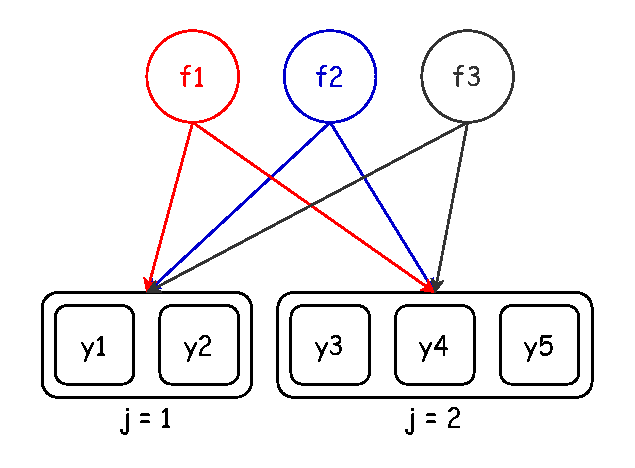
\includegraphics[width=0.48\textwidth]{figs/data_structure.drawio.pdf}
    \caption{Data Structure: Orthogonal case that each latent factors $f1$–$f3$ is independent to others. Each directed edge represents that a latent factor affects the response variable $\bm{y}_{ij}$ for $j\in\{1,2\}$. Notice that each latent factor affects all groups publicly.}
    \label{fig:data_structure}
\end{figure}

\paragraph*{Observation Level}
Conditional on the total count $y_{ij\cdot}=\sum_{q=1}^{Q}y_{ijq}$ and group-level random effect $\bm{\lambda}_{j}\in \mathbb{R}^{Q}$, each observation follows a Multinomial distribution:
\begin{equation}
    \bm{y}_{ij} \mid  y_{ij\cdot} , \bm{\lambda}_{j}
    \sim \operatorname{Multinomial}\left(y_{ij\cdot},\, \bm{p}_{ij}\right), \quad p_{ijq}=\frac{\exp(\eta_{ijq})}{\sum_{q'=1}^{Q}\exp(\eta_{ijq'})},
    \label{eq:conditional-pm}
\end{equation}
where the log-linear predictor is:
\begin{equation}
    \eta_{ijq}=\mu_{q}+\bm{v}_{ij}^{\top}\bm{\phi}_{q}+
    \lambda_{jq}, \quad q=1,2,\dots, Q,
    \label{eq:linear-predictor}
\end{equation}
and $\mu_{q}\in\mathbb{R}$ is the category-specific intercept, $\bm{\phi}_{q}\in\mathbb{R}^{P}$ is the vector of covariate effects for category $q$, and $\lambda_{jq}$ is the contribution of group $j$ to the log-relative-rate of category $q$. Equation~\eqref{eq:linear-predictor} extends the linear predictor of DMR \citep{Taddy_2015} and of the grouped Poisson-trick extension of \citet{lee2017poissontrickextensionsfitting}; the three models differ only in the distribution placed on $\bm{\lambda}_{j}$.

The softmax link in \eqref{eq:conditional-pm} is invariant under the shift $\eta_{ijq}\mapsto\eta_{ijq}+c_{ij}$ for any constant $c_{ij}$ common to all categories, so the intercepts $\bm{\mu}=(\mu_{1},\dots,\mu_{Q})$ are identified only up to an additive constant. We remove this indeterminacy by imposing the reference constraint $\mu_{1}=0$ (equivalently, a sum-to-zero constraint $\sum_{q}\mu_{q}=0$); identification is in any case restored automatically by the Poisson representation introduced below, in which each category carries its own offset.

Throughout, the total count $y_{ij\cdot}$ is treated as ancillary for $(\bm{\mu},\bm{\Phi},\bm{\lambda}_{j})$: its generating mechanism is assumed to carry no information about these parameters beyond what is already encoded in them, so that conditioning on $y_{ij\cdot}$ in \eqref{eq:conditional-pm} loses no relevant information. This is the standard convention in Multinomial regression, but it is not automatic, and we do not pursue a joint volume--composition model here. We stress that ancillarity is a statement about information, not about determinism: the total remains a random quantity, but its distribution carries no additional information about $(\bm{\mu},\bm{\Phi},\bm{\lambda}_{j})$. In Section~\ref{sec:PME} we exploit the Poisson-Multinomial equivalence to represent each $y_{ijq}$ as an independent Poisson variate whose offset $\xi_{ij}$ absorbs the (random) total; the Multinomial conditional in \eqref{eq:conditional-pm} is recovered exactly upon conditioning on $y_{ij\cdot}$. The two views are therefore consistent, and $\xi_{ij}$ is a computational device rather than a modelling assumption about the total.

\paragraph*{Group Level}

The group random effects are assumed independently and identically distributed:

\begin{equation}
    \bm{\lambda}_{j}\sim \mathcal{N}(\bm{0},\bm{\Sigma}), \quad \bm{\Sigma}=\mathbf{BB}^{\top}+\mathbf{D},
    \label{eq: Overall notation structure}
\end{equation}
where $\mathbf{B}\in \mathbb{R}^{Q\times K}$ is the factor loadings matrix and $\mathbf{D}$ is the variance. Equivalently, in the factor regression form:

\begin{equation}
    \bm{\lambda}_{j}=\mathbf{B}\mathbf{f}_{j}+\bm{\epsilon}_{j}, \quad \mathbf{f}_{j}\sim \mathcal{N}(\bm{0},\bm{I}_{K}), \quad \bm{\epsilon}_{j}\sim \mathcal{N}(\bm{0},\mathbf{D}),
    \label{eq: Detailed notation structure}
\end{equation}
so that $\lambda_{jq}=\mathbf{b}_{q}^{\top}\mathbf{f}_{j}+\epsilon_{jq}$, where $\mathbf{b}_{q}$ is the q-th row of $\mathbf{B}$. We use \ref{eq: Overall notation structure} for inference and \ref{eq: Detailed notation structure} for interpretation.

For the error matrix $\mathbf{D}$, we do the analysis with the assumption $\mathbf{D}=\sigma^{2}\mathbf{I}_{Q}$ with $\sigma^{2} >0$ instead of taking the diagonal assumption $\mathbf{D}=\text{diag}(d_{1}^{2},\dots,d_{Q}^{2})$ with entries $d_{q}>0$. The chosen form of the error is selected to simplify the computation when we introduce the Woodbury equality in Chapter~\ref{cha:}, whose result is more complex to explain in diagonal assumption.

\begin{remark}[Variance decomposition]
The variance of the log-relative-rate of category $q$ decomposes as 
\begin{equation*}
    \operatorname{Var}(\lambda_{jq})=\|\mathbf{b}_{q}\|^{2}+\sigma^{2},
\end{equation*}
where $\|\mathbf{b}_{q}\|^{2}$ captures the structured factor component and $\sigma^2$ the idiosyncratic component. The ratio $\|\mathbf{b}_{q}\|^2/(\|\mathbf{b}_{q}\|^2+\sigma^2)$ quantifies the proportion of between-group variation in category $q$ explained by the latent factors. 
\end{remark}

\section{Identifiability}
\label{sec:identifiability}

In many settings, we categorize the latent factors into orthogonal and non-orthogonal\citet{@articleCui_2026}. Orthogonal factors are assumed to be independent, which illustrates the relationship of factors in our group random effects \ref{eq: Detailed notation structure}. In this section, we present the conditions that guarantee the rotational identifiability, which are treated as given in the rest of the thesis. 

Both linear latent factor model and the generalized latent factor model suffer form rotational indeterminacy, which is the primary source of non-identification in factor analysis (\citet{BAI2012}, \citet{BAI201318}). The factor structure \ref{eq: Detailed notation structure} is subject to classical indeterminacy, which includes both rotational and sign indeterminacy. For any $K\times K$ orthogonal matrix $\mathbf{V}$, the substitution $(\mathbf{B},\mathbf{f}_{j})\to (\mathbf{BV},\mathbf{V}^{\top}\mathbf{f}_{j})$ leaves the distribution of $\bm{\lambda}_{j}$ unchanged. Also, the substitution $(\mathbf{b}_{k},\mathbf{f}_{j})\to (-\mathbf{b}_{k},-\mathbf{f}_{j})$ product of $\mathbf{b}_{q}\mathbf{f}_{k}$ is the same as $(-\mathbf{b}_{q})(-\mathbf{f}_{k})$. 

A more common approach in applications to ensure identifiability is to prescribe zeros in the loading matrix $\mathbf{B}$. Under our orthogonal assumption, the additional $K(K-1)/2$ constrains are imposed by fixing $K(K-1)/2$ entries to be zeros. Interestingly, the Example~\ref{eg:no-rotational} shows that not all configurations of the $K(K-1)/2$ zeros ensure identifiability.

\begin{example}
    This example was given by~\citet{Cui2026}. We set $K=3$ and assign at least 3 zeros in loading matrix $\mathbf{B}$. Consider the loading matrix $\mathbf{B}$ and the orthogonal transformation matrix $\mathbf{G}$,
    \begin{equation*}
        \mathbf{B}_{[1:2,]}=
        \begin{pmatrix}
            0 & a_{12} & a_{13} \\
            a_{21} & 0 & 0 
        \end{pmatrix}, \quad \mathbf{G}_{\theta}=
        \begin{pmatrix}
            1 & 0 & 0 \\
            0 & \cos \theta & \sin \theta \\
            0 & -\sin \theta & \cos \theta
        \end{pmatrix}.
    \end{equation*}
    For any $\theta$, 
    \begin{equation*}
        [\mathbf{B}\mathbf{G}_{\theta}]_{[1:2,]}
        =
        \begin{pmatrix}
            0 & *_{12} & *_{13} \\
            a_{21} & 0 & 0 
        \end{pmatrix}.
    \end{equation*}
    
    For any $\theta$, the zero pattern of $[\mathbf{B}\mathbf{G}_{\theta}]_{[1:2,]}$ retains the same as $\mathbf{B}_{[1:2,]}$. Thus, the above transformation matrix $\mathbf{G}_{\theta}$ leaves the factor covariance matrix unchanged, which is not rotationally identifiable under this constraint. 
    \label{eg:no-rotational}
\end{example}

Example~\ref{eg:no-rotational} shows that a necessary condition for identifiability is that no two columns of the loading matrix share the same zero pattern. To avoid these cases, we consider the following sufficient condition that covers many commonly used identifiability constraints. Thus, we give the positive lower triangular constraint to recover the true value of matrix $\mathbf{B}$, 

\begin{equation}
    b_{qk}=0 \text{ for } q<k,
    \label{eq: PLT1}
\end{equation}
\begin{equation}
    b_{kk}>0 \text{ for }k=1,2,\dots ,K,
    \label{eq:PLT2}
\end{equation}
which solves the rotationally indeterminacy by condition~\ref{eq: PLT1} and sign indeterminacy by condition~\ref{eq:PLT2}. \citet{Cui2026} had proved many sufficient constraints, and we adapt their IC$^{(2)}$ with orthogonal latent factors in factor analysis.


\chapter{Methodology}
\label{cha:methodology}

The observed-data log-likelihood under the model of Chapter~\ref{cha:model-specification} is

\begin{equation}
    \ell(\bm{\theta})=\sum_{j=1}^{J}\sum_{i\in \mathcal{I}_{j}}\log p(\bm{y}_{ij}\mid \bm{\theta})=\sum_{j=1}^{J}\sum_{i\in \mathcal{I}_{j}}\log \int p(\bm{y}_{ij}\mid \bm{\lambda}_{j})p(\bm{\lambda}_{j}\mid \bm{\Sigma})\,d\bm{\lambda}_{j},
    \label{eq:log-lik-chap2}
\end{equation}

where the parameter space is $\bm{\theta}:=\{\bm{\mu}, \bm{\Phi}, \mathbf{B},\sigma^{2}\}$. The integral in \ref{eq:log-lik-chap2} has no closed form, because the Gaussian prior on $\bm{\lambda}_{j}$ is not conjugate to the multinomial likelihood, so we treat $\{\bm{\lambda}_{j}\}_{j=1}^{J}$ as missing data and then estimate $\bm{\theta}=\{\bm{\mu}, \bm{\Phi}, \mathbf{B},\sigma^{2}\}$ by EM. The standard approach in generalized linear mixed models is the Laplace approximation (\citet{Breslow_1993}, \citet{Tierney01031986}), which replaced the integral with a Gaussian approximation at the posterior mode.

\section{The Choice of Approximation Level}
\label{sec:the-choice-of-approximation-level}

A natural approach motivated by the PLN-PCA model (\citet{chiquet2018variational}) approximates the posterior of the K-dimensional factor $p(\mathbf{f}_{j}\mid \bm{y}_{ij})$. Since we assumed $K\ll Q$, this reduces the Newton-step Hessian from $Q\times Q$ to $K\times K$, which appears computationally attractive. However, this approach encounters two fundamental obstacles. 

\paragraph*{Group Collapsing} Within group $j$, observations $\{i\in \mathcal{I}_{j}\}$ share the same factor $\mathbf{f}_{j}$ but carry distinct covariate vectors $\bm{v}_{ij}$ and total count $y_{ij\cdot}$. The factor-space log-posterior requires summing $\sum_{i\in \mathcal{I}_{j}}\log p(\bm{y}_{ij}\mid \mathbf{f}_{j})$, where each term involves its own normalizing constant $\sum_q \exp\bigl(\eta_{ijq}(\mathbf{f}_j)\bigr)$. A naive implementation collapses all observations in group $j$ into a single super-observation with total counts $\bm{y}_{\cdot j} = \sum_{i\in \mathcal{I}_{j}} \bm{y}_{ij}$ and averaged fixed effects $\bar{\bm{\eta}}_{j}$, treating the group as a single Multinomial draw. This is mathematically incorrect. The Multinomial log-normalizer does not linearize under summation, and the approximation error grows with within-group heterogeneity in $\bm{v}_{ij}$. 

\paragraph*{Posterior Second-Moment Deflation} The factor-space Laplace posterior yields a second-moment matrix $\mathbf{W}_{f}=J^{-1}\sum_{j}(\hat{\mathbf{f}}_{j}\hat{\mathbf{f}}_{j}^{\top}+\hat{\mathbf{V}}_{j})$ that systematically underestimates $\mathbf{I}_{K}$ due to Laplace shrinkage. Because the M-step for $\mathbf{B}$ receives only $\mathbf{BW}_{f}\mathbf{B}^{\top}$ as its sufficient statistic for $\bm{\Sigma}$, the Rubin–Thayer algorithm (\citet{Rubin1982}) compensates by inflating $\hat{\mathbf{B}}$, leading to the error in estimation. 
Thus, instead of approximate the posterior of $K$ dimensional latent factors, we do the approximation on Q dimensional group random effect $p(\bm{\lambda}_{j}\mid \bm{y}_{ij})$ directly and move the factor decomposition from the E-step to the M-step. The E-step treats $\bm{\lambda}_{j}$ as an unknown Q-vector with Gaussian prior $\mathcal{N}(\bm{0},\bm{\Sigma})$, then the M-step decomposes the resulting estimated covariance $\hat{\bm{\Sigma}}_{\text{obs}}$ into $\mathbf{BB}^{\top}+\sigma^{2}\mathbf{I}$.

\iffalse

Before we lay out our detailed EM algorithm, we introduce three technical conditions, which will significantly simplify our presentation. Different from single scalar space, our parameter space $\bm{\theta}=\{\bm{\mu}, \bm{\Phi}, \mathbf{B},\sigma^{2}\}$ given by~\ref{eq:log-lik-chap2} contains both scalar, vector and matrix.

\begin{condition}[Self-Consistency]
Function $Q(\cdot\mid \bm{\theta^{*}})$ is self-consistency, namely
\begin{equation}
    \bm{\theta^{*}}=\arg\max_{\bm{\theta}\in \Omega} Q(\bm{\theta}\mid \bm{\theta^{*}})
    \label{eq:self-consistency}
\end{equation}
\end{condition}

\begin{condition}[Strong Concavity and Smoothness]
$Q(\cdot\mid \bm{\theta^{*}})$ is strongly concave over $\Omega$, that is,
\begin{equation}
    Q(\bm{\theta}_{2}\mid \bm{\theta^{*}})-Q(\bm{\theta}_{1}\mid \bm{\theta^{*}})-\langle \nabla Q(\bm{\theta}_{1}\mid \bm{\theta^{*}}), \bm{\theta}_{2}-\bm{\theta}_{1}\rangle\leq -\frac{\gamma}{2}\|\bm{\theta}_{2}-\bm{\theta}_{1}\|^{2}, \quad \forall \bm{\theta}_{1},\bm{\theta}_{2}\in \Omega.
    \label{eq:strong-concave}
\end{equation}
$Q(\cdot\mid \bm{\theta^{*}})$ is $\mu$-smooth over $\Omega$, that is, for any $\bm{\theta}$ near $\bm{\theta}^{*}$,
\begin{equation}
    Q(\bm{\theta}_{2}\mid \bm{\theta^{*}})-Q(\bm{\theta}_{1}\mid \bm{\theta^{*}})-\langle \nabla Q(\bm{\theta}_{1}\mid \bm{\theta^{*}}), \bm{\theta}_{2}-\bm{\theta}_{1}\rangle\geq -\frac{\mu}{2}\|\bm{\theta}_{2}-\bm{\theta}_{1}\|^{2}, \quad \forall \bm{\theta}_{1},\bm{\theta}_{2}\in \Omega.
    \label{eq:smooth}
\end{equation}
\end{condition}

\begin{condition}[Gradient Stability]
    \begin{equation}
        \| \nabla Q(\mathcal{M}(\bm{\theta})\mid \bm{\theta})-\nabla Q(\mathcal{M}(\bm{\theta})\mid \bm{\theta}^{*})\|\leq \tau \|\bm{\theta}-\bm{\theta}^{*}\|
    \end{equation}
\end{condition}

\fi

\section{E-Step: Laplace Approximation}
\label{sec: E-step}
    For each group $j$, the log-posterior of $\bm{\lambda}_{j}$ is given by:
\begin{equation}
    \mathcal{L}(\bm{\lambda}_{j})=\sum_{i\in \mathcal{I}_{j}}\Bigl[\sum_{q}y_{ijq}\eta_{ijq}(\bm{\lambda}_{j})-y_{ij\cdot}\log \sum_{q}\exp\bigl(\eta_{ijq}(\bm{\lambda}_{j})\bigr)\Bigr]-\frac{1}{2}\bm{\lambda}_{j}^{\top}\bm{\Sigma}^{-1}\bm{\lambda}_{j},
    \label{eq: estep-loglik}
\end{equation}
up to an additive constant independent of $\bm{\lambda}_{j}$, where 
\begin{equation}
    \eta_{ijq}(\bm{\lambda}_{j})=\mu_{q}+\bm{v}_{ij}^{\top}\bm{\phi}_{q}+\lambda_{jq},
    \label{eq: individualcovariate}
\end{equation}
is evaluated separately for each $i\in \mathcal{I}_{j}$, gives the individual-specific covariate structure.
The gradient and Hessian of \ref{eq: estep-loglik} are

\begin{equation}
    \nabla_{\bm{\lambda}_{j}}\ell=\sum_{i\in \mathcal{I}_{j}}\bigl(\bm{y}_{ij}-y_{ij\cdot}\bm{p}_{ij}(\bm{\lambda}_{j})\bigr)-\bm{\Sigma}^{-1}\bm{\lambda}_{j},
\end{equation}

\begin{equation}
    \mathbf{H}(\bm{\lambda}_{j})=-\sum_{i\in\mathcal{I}_{j}}y_{ij\cdot}\mathbf{P}_{ij}(\bm{\lambda}_{j})-\bm{\Sigma}^{-1},
        \label{eq: hessian-equality}
\end{equation}
where $\bm{p}_{ij}(\bm{\lambda}_{j})=\operatorname{softmax}\bigl(\bm{\eta}_{ij}(\bm{\lambda}_{j})\bigr)$ and $\mathbf{P}_{ij}=\text{diag}(\bm{p}_{ij})-\bm{p}_{ij}\bm{p}_{ij}^{\top}$. Since $\mathbf{P}_{ij}\succeq 0$ and $\bm{\Sigma}^{-1}\succ 0$, we have $\mathbf{H}(\bm{\lambda}_{j})\prec 0$ everywhere, so $\ell(\bm{\lambda}_{j})$ is strictly concave and has a unique maximizer

\begin{equation}
     \hat{\bm{\lambda}}_{j}
     = \arg\max_{\bm{\lambda}\in \mathbb{R}^{Q}}
     \ell_{j}(\bm{\lambda}_{j}).
     \label{eq:maximizer}
\end{equation}

Newton's method

\begin{equation}
    \bm{\lambda}_{j}^{(t+1)}=
    \bm{\lambda}_{j}^{(t)}
    -s^{(t)}\mathbf{H}\bigl(\bm{\lambda}_{j}^{(t)}
    \bigr)^{-1}\nabla_{\bm{\lambda}_{j}}
    \ell \bigl(\bm{\lambda}_{j}^{(t)}\bigr),
    \label{eq:newton-method}
\end{equation}
with backtracking step size $s^{(t)}$ converges to the unique global maximum $\hat{\bm{\lambda}}_{j}$ from any initialization. The Laplace approximation then yields

\begin{equation}
    p(\bm{\lambda}_{j}\mid \bm{y}_{ij}) \approx \mathcal{N}\bigl(\hat{\bm{\lambda}}_{j}, \hat{\mathbf{S}}_{j}\bigr), \quad \hat{\mathbf{S}}_{j}=\bigl(-\mathbf{H}(\hat{\bm{\lambda}_{j}})\bigr)^{-1}.
    \label{eq:surrogate-eq}
\end{equation}

\section{M-Step (a): Fixed Effects via Poisson GLMs}
\label{sec:M-step(a)}

    With $\hat{\bm{\lambda}}_{j}$ fixed, recompute the Poisson-Multinomial Equivalence offset:
\begin{equation}
    \xi_{ij}=\log y_{ij\cdot}-\log \sum_{q}\exp\bigl(\hat{\mu}_{q}+\bm{v}_{ij}^{\top}\hat{\bm{\phi}}_{q}+\hat{\lambda}_{jq}\bigr).
\end{equation}
For $q=1,2,\dots,Q$, we solve the maximization problem independently:
\begin{equation}
    (\hat{\mu}_{q}, \hat{\bm{\phi}}_{q})=\arg \max_{\mu_{q}, \bm{\phi}_{q}}\sum_{i}\bigl[y_{ijq}(\mu_{q}+\bm{v}_{ij}^{\top}\bm{\phi}_{q})-\exp (\mu_{q}+\bm{v}_{ij}^{\top}\bm{\phi}_{q}+\hat{\lambda}_{jq}+\xi_{ij})\bigr].
\end{equation}
This is a Poisson log-linear regression with offset $\lambda_{jq}+\xi_{ij}$, solved by iteratively reweighted least squares. The Q problems are independent and may be parallelized. 

\section{M-Step (b): Factor Loadings and Idiosyncratic Variance}
\label{sec:M-step(b)}

The EM sufficient statistic for $\bm{\Sigma}$ follows directly from the Laplace output:

\begin{equation}
    \hat{\bm{\Sigma}}_{\text{obs}}=\frac{1}{J}\sum_{j}\mathbb{E}[\bm{\lambda}_{j} \bm{\lambda}_{j}^{\top}\mid \bm{y}_{ij}]\approx \frac{1}{J}\sum_{j}(\hat{\bm{\lambda}}_{j} \hat{\bm{\lambda}}_{j}^{\top}+\hat{\mathbf{S}}_{j}).
    \label{eq:sigma-obs}
\end{equation}

Critically, $\hat{\bm{\Sigma}}_{\text{obs}}$ is fully determined by current Laplace output $(\hat{\bm{\lambda}}_{j}, \hat{\mathbf{S}}_{j})$ and does not need to be re-evaluated during the Rubin-Thayer sub-iterations, thus eliminating the circular dependency inherent in factor-space formulations.
Given $\hat{\bm{\Sigma}}_{\text{obs}}$, we decompose $\bm{\Sigma}=\mathbf{BB}^{\top}+\sigma^2\mathbf{I}_{Q}$ via the Rubin-Thayer EM factor analysis algorithm (\citet{Rubin1982})

\begin{equation}
\hat{\boldsymbol{\beta}}
=
\hat{\mathbf{B}}^\top
\left(
\hat{\mathbf{B}}\hat{\mathbf{B}}^\top
+
\hat{\sigma}^2 \mathbf{I}_Q
\right)^{-1},
\label{eq: Rubin1}
\end{equation}
\begin{equation}
\hat{\boldsymbol{\Theta}}
=
\mathbf{I}_{K}
-
\hat{\boldsymbol{\beta}}\hat{\mathbf{B}}
+
\hat{\boldsymbol{\beta}}
\hat{\boldsymbol{\Sigma}}_{\mathrm{obs}}
\hat{\boldsymbol{\beta}}^\top,
\label{eq: Rubin2}
\end{equation}
\begin{equation}
\hat{\mathbf{B}}_{\mathrm{new}}
=
\hat{\boldsymbol{\Sigma}}_{\mathrm{obs}}
\hat{\boldsymbol{\beta}}^\top
\hat{\boldsymbol{\Theta}}^{-1},
\label{eq: Rubin3}
\end{equation}
\begin{equation}
\hat{\sigma}_{\mathrm{new}}^{2}
=
\frac{1}{Q}
\operatorname{tr}
\left(
\hat{\boldsymbol{\Sigma}}_{\mathrm{obs}}
-
\hat{\mathbf{B}}_{\mathrm{new}}
\hat{\boldsymbol{\beta}}
\hat{\boldsymbol{\Sigma}}_{\mathrm{obs}}
\right).
\label{eq: Rubin4}
\end{equation}

The iterations  \ref{eq: Rubin1}-\ref{eq: Rubin4} are repeated to convergence. The PLT constraint \ref{eq: PLT} is enforced post-hoc via a QR decomposition of the top K rows of $\hat{\mathbf{B}}_{\text{new}}$, followed by sign correction to ensure positive diagonal entries and zeroing of the upper triangle. Applying PLT only after the Rubin–Thayer sub-iterations converge, rather than at each inner step, avoids the discontinuities that would otherwise disrupt convergence.
    Given $\hat{\mathbf{B}}$ and $\hat{\sigma}^2$, the factor scores are recovered by the Bayes linear estimator (\citet{Gelman2013}):
\begin{equation}
\hat{\mathbf{f}}_j = \left( \mathbf{I}_K + \frac{1}{\hat{\sigma}^2} \hat{\mathbf{B}}^\top \hat{\mathbf{B}} \right)^{-1} \frac{1}{\hat{\sigma}^2} \hat{\mathbf{B}}^\top \hat{\boldsymbol{\lambda}}_j ,
\label{eq: Bayeslinearestimator}
\end{equation}
requiring only $K\times K$ inversion via Woodbury equality.

\section{Convergence}
\label{sec:convergence}




% \chapter{Computational Acceleration for Large-Q Regime}
\label{cha:computational-acceleration}

Chapter~\ref{cha:methodology} derived a correct and convergent Laplace-EM algorithm, but left its dominant per-iteration cost unaddressed. Each Newton step in E-step~\ref{sec: E-step} requires forming and solving the $Q\times Q$ system~\ref{eq: hessian-equality} at cost $\mathcal{O}(N_{j}Q^{2}+Q^{3})$, in the meanwhile, each inner iteration of the M-step factor update~\ref{eq: Rubin3}-\ref{eq: Rubin4} requires forming $\bm{\Sigma}^{-1}$ densely at cost $\mathcal{O}(Q^{3})$. For large Q, these costs are not merely inconvenient but make the algorithm impractical. This chapter develops an exact acceleration method to remove this bottleneck by showing that the Poisson-Multinomial equivalence that already underlies the M-step can be redeployed via auxiliary-variable construction, which can remove the cross-category coupling from the E-step Hessian as well. 

\section{PME Auxiliary-Variable Construction}
\label{sec:auxiliary-variable-construction}

For a fixed group $j$, we introduce an auxiliary scalar $\xi_{i}$ per observation $i\in \mathcal{I}_{j}$ and define the Poisson surrogate log-posterior
\begin{equation}
    \ell_P(\boldsymbol{\lambda}, \boldsymbol{\xi}) \;=\; \sum_{i \in \mathcal{I}_j} \sum_{q=1}^{Q} \Big[ y_{iq}\, \eta_{iq}(\boldsymbol{\lambda}) - \exp\big(\eta_{iq}(\boldsymbol{\lambda}) + \xi_i\big) \Big] \;-\; \tfrac{1}{2} \boldsymbol{\lambda}^\top \boldsymbol{\Sigma}^{-1} \boldsymbol{\lambda},
\end{equation}
which treats the counts as independent Poisson draws with rate $\exp{(\eta_{iq}+\xi_{i})}$ rather than as a multinomial draw. This is the same auxiliary-variable idea that underlies Proposition~\ref{prop:PME}, but it is now applied to the E-step posterior instead of M-step likelihood.

\section{Diagonal Low Rank Hessian \& Woodbury Solve}
\label{sec:diagonal-low-rank-hessian}

With $\bm{\xi}$ fixed at $\bm{\xi}^{*}(\bm{\lambda})$, we denote $d_{q}:=\sum_{i\in \mathcal{I}_{j}}\exp{\bigl(\eta_{iq}(\bm{\lambda})+\xi_{i}\bigr)}$. The Hessian of $\ell_{P}(\cdot, \bm{\xi})$ with respect to $\bm{\lambda}$ is 
\begin{equation}
    \mathbf{H}_{P}(\bm{\lambda})=-\text{diag}(\mathbf{d})-\bm{\Sigma}^{-1}, \quad \mathbf{d}=(d_{1},\dots, d_{Q})^{\top},
    \label{eq:acceleration-hessian1}
\end{equation}
which is purely diagonal in its Poisson part. We expand $\bm{\Sigma}^{-1}$ by the Woodbury identity

\begin{equation}
    \bm{\Sigma}^{-1}=\sigma^{-2}\mathbf{I}_{Q}-\sigma^{-4}\mathbf{BM}_{K}^{-1}\mathbf{B}^{\top} \text{ with } \mathbf{M}_{K}=\mathbf{I}_{K}+\sigma^{-2}\mathbf{B}^{\top}\mathbf{B}.
    \label{eq:woodbury2}
\end{equation}

We write $\tilde{\mathbf{D}}=\text{diag}(\mathbf{d}+\sigma^{-2}\mathbf{1}_{Q})$ for the combined diagonal term
\begin{equation}
    -\mathbf{H}_{P}(\bm{\lambda})=\tilde{\mathbf{D}}-\sigma^{-4}\mathbf{BM}_{K}^{-1}\mathbf{B}^{\top},
    \label{eq:acceleration-hessian3}
\end{equation}
it's a $Q\times Q$ matrix. Applying Woodbury identity once more and we obtain
\begin{equation}
    \bigl(-\mathbf{H}_{P}(\bm{\lambda})\bigr)^{-1}=\tilde{\mathbf{D}}^{-1}-\tilde{\mathbf{D}}^{-1}\mathbf{B}\bm{\Gamma}^{-1}\mathbf{B}^{\top}\tilde{\mathbf{D}}^{-1} \text{ with } \bm{\Gamma}:=\mathbf{B}^{\top}\tilde{\mathbf{D}}^{-1}\mathbf{B}-\sigma^{4}\mathbf{M}_{K}.
    \label{eq:inverse-hessian4}
\end{equation}

Therefore, given the Cholesky factor $\mathbf{L}$ of $-\bm{\Gamma}$, a Newton direction $\Delta\bm{\lambda}=\bigl(-\mathbf{H}_{P}(\bm{\lambda})\bigr)^{-1}\mathbf{g}$ for any gradient vector $\mathbf{g}$ is obtained as

\begin{equation}
    \Delta\boldsymbol{\lambda} \;=\; \tilde{\mathbf{D}}^{-1}\mathbf{g} \;+\; \tilde{\mathbf{D}}^{-1}\mathbf{B}(\mathbf{L}\mathbf{L}^\top)^{-1}\mathbf{B}^\top\tilde{\mathbf{D}}^{-1}\mathbf{g},
    \label{eq:newton-direction5}
\end{equation}
computed by two matrix-vector products against $\mathbf{B}$ and one $K\times K$ triangular solve, after a one-time $\mathcal{O}(QK^{2}+K^{3})$ cost to form $\bm{\Gamma}$ and its Cholesky factor.

\begin{proposition}[Negative definiteness and conditioning of $\bm{\Gamma}$]
    \label{prop:negative-definiteness}
    If $\bm{\Gamma}\prec 0$ and $\lambda_{\text{max}}(\bm{\Gamma})\leq -\sigma^{4}$, then $-\bm{\Gamma}\succ \sigma^{4}\mathbf{I}_{K}$ uniformly in $\bm{\lambda}$, $\mathbf{B}$ and data.
    \label{prop:negative-definiteness}
\end{proposition}

\begin{proof}
    Since $d_{q}\geq 0$ for each $q$, $\tilde{\mathbf{D}}=\text{diag}(\mathbf{d}+\sigma^{-2}\mathbf{1}_{Q})\succeq \sigma^{-2}\mathbf{I}_{Q}$. Therefore, $\tilde{\mathbf{D}}^{-1}\preceq \sigma^{2}\mathbf{I}_{Q}$ and $\mathbf{B}^{\top}\tilde{\mathbf{D}}^{-1}\mathbf{B}\preceq \sigma^{2}\mathbf{B}^{\top}\mathbf{B}$.
    Rewrite the definition of $\bm{\Gamma}$ in~\ref{eq:inverse-hessian4} using the substitution $\mathbf{M}_{K}=\mathbf{I}_{K}+\sigma^{-2}\mathbf{B}^{\top}\mathbf{B}$, then
    \[
        -\bm{\Gamma}=\sigma^{4}\mathbf{M}_{K}-\mathbf{B}^{\top}\tilde{\mathbf{D}}^{-1}\mathbf{B}\succeq \sigma^{4}\mathbf{M}_{K}+\sigma^{2}\mathbf{B}^{\top}\mathbf{B}-\sigma^{2}\mathbf{B}^{\top}\mathbf{B}=\sigma^{4}\mathbf{I}_{K}.
    \]
\end{proof}

Proposition~\ref{prop:negative-definiteness} guarantees that the Cholesky factorization used in~\ref{eq:newton-direction5} is always numerically well behaved. Regardless of how large $Q$ and $\mathbf{B}$ increase, the relevant $K\times K$ matrix never becomes ill-conditioned purely as an artefact of dimension, since its smallest eigenvalue is bounded below by the dimension-free quantity $\sigma^{4}$.

\section{Ascent Direction on True Posterior}
\label{sec:ascent-direction-on-true-posterior}

The direction $\Delta \bm{\lambda}$ of~\ref{eq:newton-direction5} is a Newton step for the surrogate objective $\ell_{P}(\cdot, \bm{\xi}^{*}\bigl(\bm{\lambda})\bigr)$ instead of true log-posterior $\ell$.

\begin{algorithm}[t]
    \caption{E-step inner iteration: posterior-mode search for the group effect $\bm{\lambda}_j$}
    \label{alg:estep-inner}
    \begin{algorithmic}[1]
    \Require group data $\{\bm{y}_{ij}\}_{i\in\mathcal{I}_j}$; current parameters
         $(\bm{\mu},\bm{\Phi},\mathbf{B},\sigma^2)$; Armijo constants
         $c_1\in(0,1)$, $\rho\in(0,1)$; tolerance $\epsilon>0$
    \Ensure posterior mode $\widehat{\bm{\lambda}}_j$ and curvature $-\mathbf{H}(\widehat{\bm{\lambda}}_j)$
    \State initialize $\bm{\lambda}^{(0)}\gets \mathbf{0}$;\quad $t\gets 0$
    \Repeat
    \State re-profile the offset $\bm{\xi}^{(t)}\gets \bm{\xi}(\bm{\lambda}^{(t)})$
    \State $\mathbf{g}^{(t)}\gets \nabla\ell(\bm{\lambda}^{(t)})$
    \State form $-\mathbf{H}_P(\bm{\lambda}^{(t)})
         =\bar{\mathbf{D}}^{(t)}-\sigma^{-4}\mathbf{B}\mathbf{M}_K^{-1}\mathbf{B}^\top$
    \State solve $\bigl(-\mathbf{H}_P(\bm{\lambda}^{(t)})\bigr)\,\Delta\bm{\lambda}^{(t)}=\mathbf{g}^{(t)}$
    \State $s^{(t)}\gets 1$
    \While{$\ell\bigl(\bm{\lambda}^{(t)}+s^{(t)}\Delta\bm{\lambda}^{(t)}\bigr)
          < \ell(\bm{\lambda}^{(t)})+c_1\,s^{(t)}\,\mathbf{g}^{(t)\top}\Delta\bm{\lambda}^{(t)}$}
    \State $s^{(t)}\gets \rho\,s^{(t)}$
    \EndWhile
    \State $\bm{\lambda}^{(t+1)}\gets \bm{\lambda}^{(t)}+s^{(t)}\Delta\bm{\lambda}^{(t)}$;\quad
         $t\gets t+1$
    \Until{$\lVert\mathbf{g}^{(t)}\rVert\le \epsilon$}
    \State $\widehat{\bm{\lambda}}_j\gets \bm{\lambda}^{(t)}$
    \State \Return $\widehat{\bm{\lambda}}_j$ and
       $-\mathbf{H}(\widehat{\bm{\lambda}}_j)$
    \end{algorithmic}
    \end{algorithm}

\begin{lemma}[Ascent direction]
    Let $\mathbf{g}=\nabla \ell(\bm{\lambda})$ and $\Delta \bm{\lambda}=\bigl(-\mathbf{H}_{P}(\bm{\lambda})\bigr)^{-1}\mathbf{g}$. If $\mathbf{g}\neq \bm{0}$, then $\mathbf{g}^{\top}\Delta \bm{\lambda}>0$.
\end{lemma}

\begin{proof}
    Since $\bm{\Gamma}\prec 0$ implies the Woodbury-expanded matrix in~\ref{eq:inverse-hessian4} is positive definite. Equivalently, \ref{eq:acceleration-hessian3} is positive definite because it is the negative Hessian of the strictly concave function $\ell_{P}(\cdot, \bm{\xi})$. Hence, $-\mathbf{H}_{P}(\bm{\lambda})=\tilde{\mathbf{D}}-\sigma^{-4}\mathbf{BM}_{K}^{-1}\mathbf{B}^{\top}\succ 0$ by Proposition~\ref{prop:negative-definiteness}, so its inverse is also positive definite and $\mathbf{g}^{\top}\Delta\bm{\lambda}=\mathbf{g}^{\top}\bigl(-\mathbf{H}_{P}(\bm{\lambda})\bigr)^{-1}\mathbf{g}>0$ for any $\mathbf{g}\neq 0$.
\end{proof}

Let $\ell: \mathbb{R}^{Q}\to \mathbb{R}$ denote the true conditional log-posterior of the group effect $\bm{\lambda}$, whose mode is defined by~\ref{eq:maximizer}, and $\ell_{P}(\cdot,\bm{\xi})$ denotes the Poisson surrogate log-posterior with offset $\bm{\xi}$. The Newton-type direction is 

\begin{equation}
    \Delta \bm{\lambda}=\bigl(-\mathbf{H}_{P}(\bm{\lambda})\bigr)^{-1}\mathbf{g}, \quad \mathbf{g}=\nabla\ell(\bm{\lambda}),
    \label{eq:newton-type-direction}
\end{equation}
where $\mathbf{H}_{P}(\bm{\lambda})=\nabla^{2}\ell_{P}(\bm{\lambda},\bm{\xi})$ is the Hessian of the Poisson surrogate by the Woodbury expansion~\ref{eq:acceleration-hessian3}. We propose two regularity facts on which the analysis rests, and both of them are consequences of results already established for the model.

\begin{assumption}[Curvature of true objective]
    Let $\ell\in C^{2}(\mathbb{R}^{Q})$. On initial superlevel set $\mathcal{L}_{0}:=\{\bm{\lambda}\in\mathbb{R}^{Q}:\ell(\bm{\lambda})\geq \ell(\bm{\lambda}^{(0)})\}$, there exist constants $0<\mu_{0}\leq L_{0}<\infty$ with
    \begin{equation}
        \mu_{0}\preceq -\nabla^{2}\ell(\bm{\lambda})\preceq L_{0}\mathbf{I},
    \end{equation}
    for all $\bm{\lambda}\in\mathcal{L}_{0}$.
    \label{as:ell}
\end{assumption}

Assumption~\ref{as:ell} holds for the model. The strong-concavity bound is supplied by
the Gaussian random-effect prior alone. Since $\bm{\alpha}\sim N(\mathbf 0,\bm{\Sigma})$ with
$\bm{\Sigma}=\mathbf{B}\mathbf{B}^{\top}+\sigma^{2}\mathbf{I}$, the prior contributes
$\bm{\Sigma}^{-1}\succeq(\theta_{1}+\sigma^{2})^{-1}\mathbf{I}$ to $-\nabla^{2}\ell$, so
$\mu_{0}=(\theta_{1}+\sigma^{2})^{-1}>0$ holds unconditionally.
The smoothness bound is supplied by the multinomial log-likelihood, which has
negative semi-definite curvature and whose operator norm is dominated by the total observed count
$\bigl\lVert\nabla^{2}\log p(\bm{y}\mid\bm{\lambda})\bigr\rVert\le\sum_{i}y_{ij\cdot}<\infty$, so
$L_{0}=\lambda_{\max}(\bm{\Sigma}^{-1})+\sum_{i}y_{ij\cdot}$ is finite whenever the data are finite.
Thus $\ell$ is $\mu_{0}$-strongly concave and $L_{0}$-smooth by construction, and no additional
sampling assumption is needed; the same fact guarantees that the maximizer $\hat{\bm{\lambda}}$
exists and unique, and $\mathcal{L}_{0}$ is compact.

\begin{assumption}[Uniform conditioning of the preconditioner]
    There exist constants $0<m\leq M<\infty$ independent of $t$ such that every preconditioner generated by Algorithm~\ref{alg:estep-inner} satisfies,
    \begin{equation}
        m\mathbf{I}\preceq -\mathbf{H}_{P}(\bm{\lambda}^{(t)})\preceq M\mathbf{I},
    \end{equation}
    for all iteration t.
    \label{as:prec}
\end{assumption}
Assumption~\ref{as:prec} likewise follows from the model, subject to one mild and checkable
condition on the data. The lower bound $m$ is structural: by Proposition~4.2.1 the
Woodbury-expanded matrix~\eqref{eq:woodbury} is positive definite because $\bm{\Gamma}\prec\mathbf 0$,
uniformly over the parameter region of interest. The upper bound $M$ requires that the diagonal
working weights and the profiled offset stay bounded along the iterates; the working weights
already satisfy $d_{q}\le\sum_{i}M_{i}$, so the only quantity that could degrade the conditioning
is the profiled offset $\xi_{ij}$, which enters through $\log y_{ij\cdot}$ and diverges only if a
unit carries no counts at all. It therefore suffices that every included unit has at least one
nonzero count,
\[
y_{ij\cdot}=\sum_{q=1}^{Q}y_{ijq}\ \ge\ 1\qquad\text{for all included }(i,j),
\]
under which $\xi_{ij}$ is finite and, being a continuous function of $\bm{\lambda}$
(Proposition~4.1.1) on the compact super-level set $\mathcal{L}_{0}$, keeps the spectrum of
$-\mathbf{H}_{P}(\bm{\lambda}^{(t)})$ within a fixed interval $[m,M]$. This condition is innocuous
in practice: empty units carry no information and are routinely removed during pre-processing of
count and compositional data, and the same effect is achieved by the standard pseudo-count or
truncation adjustments used for sparse counts. Assumption~\ref{as:prec} thus holds for any dataset
after the elementary pre-processing already standard in this setting.
    
\begin{lemma}[Ascent Direction]
    Let $\mathbf{g}=\nabla\ell(\bm{\lambda})$ and $\Delta \bm{\lambda}=\bigl(-\mathbf{H}_{P}(\bm{\lambda})\bigr)^{-1}\mathbf{g}$ as in~\ref{eq:newton-type-direction}. If $\mathbf{g}\neq \bm{0}$, $\mathbf{g}^{\top}\Delta\bm{\lambda}>0$. Moreover, the angle between $\Delta\bm{\lambda}$ and $\mathbf{g}$ is bounded away from a right angle,
    \begin{equation}
        \frac{\mathbf{g}^{\top}\Delta\bm{\lambda}}{\|\mathbf{g}\|\|\Delta\bm{\lambda}\|}\geq \frac{m}{M}>0.
    \end{equation}
    \label{lem:ascent-direction}
\end{lemma}

\begin{proof}
    By Assumption~\ref{as:prec}, $-\mathbf{H}_{P}(\bm{\lambda})$ is symmetric positive definite, so its inverse is symmetric positive definite as well with spectrum contained in $[M^{-1}, m^{-1}]$. Hence, for any $\mathbf{g}\neq \bm{0}$,
    \begin{equation}
        \mathbf{g}^{\top}\Delta\bm{\lambda}=\mathbf{g}^{\top}\bigl(-\mathbf{H}_{P}(\bm{\lambda})\bigr)^{-1}\mathbf{g}\geq M^{-1}\|\mathbf{g}\|^{2}>0,
    \end{equation}
    which is the first claim. For the angle, using $\mathbf{g}^{\top}\bigl(-\mathbf{H}_{P}(\bm{\lambda})\bigr)^{-1}\mathbf{g}\geq M^{-1}\|\mathbf{g}\|^{2}$ and $\|\Delta\bm{\lambda}\|=\|\bigl(-\mathbf{H}_{P}(\bm{\lambda})\bigr)^{-1}\mathbf{g}\|\leq m^{-1}\|\mathbf{g}\|$,
    \begin{equation}
        \frac{\mathbf{g}^{\top}\Delta\bm{\lambda}}{\|\mathbf{g}\|\|\Delta\bm{\lambda}\|}\geq\frac{M^{-1}\|\mathbf{g}\|^{2}}{m^{-1}\|\mathbf{g}\|^{2}}= \frac{m}{M}>0.
    \end{equation}
\end{proof}

\begin{theorem}[Global Linear Convergence under Armijo Backtracking]
    Let $\bm{\lambda}^{(0)}\in \mathbb{R}^{Q}$ be arbitrary and generate $\bm{\lambda}^{(t+1)}=\bm{\lambda}^{(t)}+s^{(t)}\Delta \bm{\lambda}^{(t)}$, where $\Delta \bm{\lambda}^{(t)}$ is computed from~\ref{eq:newton-direction5} at $\bm{\lambda}^{(t)}$. For fixed Armijo parameters $c_{1}\in(0,1)$ and $\rho\in (0,1)$, the step size $s^{(t)}=\rho^{k_{t}}$ is chosen with $k_{t}\in \{0,1,2,\cdots\}$, which is the smallest integer satisfying the sufficient-increase condition,
    \begin{equation}
        \ell(\bm{\lambda}^{(t)}+s^{(t)}\Delta \bm{\lambda}^{(t)})\geq \ell(\bm{\lambda}^{(t)})+c_{1}s^{(t)}\mathbf{g}^{(t)\top}\Delta \bm{\lambda}^{(t)},
        \label{eq:thm1-1}
    \end{equation}
    where $\mathbf{g}^{(t)}:=\nabla\ell(\bm{\lambda}^{(t)})$. Then the iterates converge to the unique maximizer $\hat{\bm{\lambda}}$ of $\ell$ at a linear rate under Assumption~\ref{as:ell}-\ref{as:prec}. That is, there exists a constant $\kappa\in (0,1]$ depending only on $(\mu_{0},L_{0},m,M,c_{1},\rho)$ such that,
    \begin{equation}
        \ell(\hat{\bm{\lambda}})-\ell(\bm{\lambda}^{(t)})\leq (1-\kappa)^{t}[\ell(\hat{\bm{\lambda}})-\ell(\bm{\lambda}^{(0)})],
        \label{eq:thm1-2}
    \end{equation}
    and,
    \begin{equation}
        \|\hat{\bm{\lambda}}-\bm{\lambda}^{(t)}\|\leq (1-\kappa)^{\frac{t}{2}}\sqrt{\frac{2}{\mu_{0}}[\ell(\hat{\bm{\lambda}})-\ell(\bm{\lambda}^{(0)})]}.
        \label{eq:thm1-3}
    \end{equation}
    \label{thm:convergence}
\end{theorem}

\begin{proof}
    If $\mathbf{g}^{(t)}=\bm{0}$ for some $t$, then $\bm{\lambda}^{(t)}$ is a stationary point of the strictly concave $\ell$, hence $\bm{\lambda}^{(t)}=\hat{\bm{\lambda}}$ and the assertion holds trivially. Under generation assumption, we assume $\mathbf{g}^{(t)}\neq \bm{0}$ and proceed the proof in four steps.
    \medskip

    \noindent\textbf{Step 1.} By Lemma~\ref{lem:ascent-direction}, $\Delta\bm{\lambda}^{(t)}$ is an ascent direction and $\mathbf{g}^{(t)\top}\Delta\bm{\lambda}^{(t)}>0$. Assumption~\ref{as:ell} gives $L_{0}$-Lipschitz continuity of $\nabla\ell$ on $\mathcal{L}_{0}$. Also, the property of monotonicity (proved below) of $\{\ell(\bm{\lambda}^{(t)})\}$ keeps every iterate in $\mathcal{L}_{0}$. Thus, the quadratic lower bound,
    \begin{equation}
        \ell(\bm{\lambda}^{(t)}+s\Delta \bm{\lambda}^{(t)})\geq \ell(\bm{\lambda}^{(t)})+s\mathbf{g}^{(t)\top}\Delta \bm{\lambda}^{(t)}-\frac{L_{0}s^{2}}{2}\|\Delta \bm{\lambda}^{(t)}\|^{2},
        \label{eq:step1-1}
    \end{equation}
    holds for all admissible $s$. Comparing~\ref{eq:step1-1} with~\ref{eq:thm1-1}, the Armijo condition is implied whenever 
    \begin{equation}
        s\leq \frac{2(1-c_{1})\mathbf{g}^{(t)\top}\Delta \bm{\lambda}^{(t)}}{L_{0}\|\Delta \bm{\lambda}^{(t)}\|^{2}}.
        \label{eq:step1-2}
    \end{equation}
    Since backtracking multiplies the trial step by $\rho$ until acceptance and starts from 1, the accepted step satisfies,
    \begin{equation}
        s^{(t)}\geq \min \left\{1,\frac{2\rho(1-c_{1})\mathbf{g}^{(t)\top}\Delta \bm{\lambda}^{(t)}}{L_{0}\|\Delta \bm{\lambda}^{(t)}\|^{2}}\right\}.
        \label{eq:step1-3}
    \end{equation}
    For the simplicity of the notation, we write $P^{(t)}=\bigl(-\mathbf{H}_{P}(\bm{\lambda})\bigr)^{-1}$ with spectrum in $[M^{-1},m^{-1}]$. From Lemma~\ref{lem:ascent-direction}, we have,
    \begin{equation}
        \frac{\mathbf{g}^{(t)\top}\Delta\bm{\lambda}^{(t)}}{\|\Delta\bm{\lambda}^{(t)}\|^{2}}\geq\frac{m^{2}}{M},
        \label{eq:step1-4}
    \end{equation}
    and hence,
    \begin{equation}
        s^{(t)}\geq s_{\min} :=\min \left\{1,\frac{2\rho(1-c_{1})m^{2}}{L_{0}M}\right\}>0,
        \label{eq:step1-5}
    \end{equation}
    which is the bound independent of $t$. In particular, the line search terminates after finitely many backtracking steps.
    \medskip

    \noindent\textbf{Step 2.} Combining the accepted Armijo inequality~\ref{eq:thm1-1} with~\ref{eq:step1-5} and $\mathbf{g}^{\top}\Delta\bm{\lambda}\geq M^{-1}\|\mathbf{g}\|^{2}$, we have,
    \begin{equation}
        \ell(\bm{\lambda}^{(t+1)})-\ell(\bm{\lambda}^{(t)})\geq c_{1}s^{(t)}\mathbf{g}^{(t)\top}\Delta \bm{\lambda}^{(t)} \geq \frac{c_{1}s_{\min}}{M}\|\mathbf{g}^{(t)}\|^{2}.
        \label{eq:step2-1}
    \end{equation}
    We define the positive constant term $\gamma:=\dfrac{c_{1}s_{\min}}{M}$. Thus, $\{\ell(\bm{\lambda}^{(t)})\}$ is non-decreasing and bounded above by $\ell{(\hat{\bm{\lambda})}}$. It converges and every iterate lies in $\mathcal{L}_{0}$, which justify the use of Assumptions~\ref{as:ell}-\ref{as:prec} and of~\ref{eq:thm1-1} above.
    \medskip

    \noindent\textbf{Step 3.} Assumption~\ref{as:ell} yields the strong concavity. That is, for every $\bm{\lambda}\in\mathcal{L}_{0}$, the quadratic upper bound satisfies that
    \begin{equation}
        \ell(\bm{y})\leq \ell(\bm{\lambda})^{\top}(\bm{y}-\bm{\lambda})-\frac{\mu_{0}}{2}\|\bm{y}-\bm{\lambda}\|^{2},
        \label{eq:step3-1}
    \end{equation}
    which maximize the right-hand side over $\bm{y}\in\mathbb{R}^{Q}$. By Polyak-Lojasiewicz inequality, we have,
    \begin{equation}
        \ell(\hat{\bm{\lambda}})-\ell(\bm{\lambda})\leq \frac{1}{2\mu_{0}}\|\nabla\ell(\bm{\lambda})\|^{2}.
        \label{eq:step3-2}
    \end{equation}
    Let $\delta_{t}:=\ell(\hat{\bm{\lambda}})-\ell(\bm{\lambda})\geq 0$. Substracting~\ref{eq:step2-1} from \ref{eq:step3-1} from $\ell(\bm{\lambda})$ and applying \ref{eq:step3-2} at $\bm{\lambda}^{(t)}$,
    \begin{equation}
        \delta_{t+1}=\delta_{t}-\left[\ell(\bm{\lambda}^{(t+1)})-\ell(\bm{\lambda}^{(t)})\right]\leq \delta_{t}-\gamma \|\mathbf{g}^{(t)}\|^{2}\leq \delta_{t}-2\gamma \mu_{0} \delta_{t}=(1-\kappa)\delta_{t},
        \label{eq:step3-3}
    \end{equation}
    where $\kappa:=2\gamma\mu_{0}=\dfrac{2c_{1}s_{\min}\mu_{0}}{M}$. Since $\delta_{t}\geq0$, $\kappa\in(0,1]$ and $\delta_{t}\leq (1-\kappa)^{t}\delta_{0}$, which is the first stated bound and shows $\ell(\hat{\bm{\lambda}})\to\ell(\bm{\lambda})$.
    \medskip

    \noindent\textbf{Step 4.} Strong concavity also gives $\ell(\hat{\bm{\lambda}})\leq\ell(\bm{\lambda})-\dfrac{\mu_{0}}{2}\|\hat{\bm{\lambda}}-\bm{\lambda}\|^{2}$. Hence, 
    \begin{equation}
        \dfrac{\mu_{0}}{2}\|\hat{\bm{\lambda}}-\bm{\lambda}^{(t)}\|^{2}\leq \delta_{t}\leq (1-\kappa)^{t}\delta_{0},
        \label{eq:step4-1}
    \end{equation}
    then,
    \begin{equation}
        \|\hat{\bm{\lambda}}-\bm{\lambda}^{(t)}\|\leq (1-\kappa)^{\frac{t}{2}}\sqrt{\frac{2\delta_{0}}{\mu_{0}}}\to 0.
        \label{eq:step4-2}
    \end{equation}
    Therefore, $\bm{\lambda}^{(t)}\to \hat{\bm{\lambda}}$, which is the unique maximizer of $\ell$.
\end{proof}

\begin{remark}
    The backtracking condition in Theorem~\ref{thm:convergence} is on the true posterior $\ell$ instead of checking on the surrogate $\ell_{P}$. It guarantees that no majorization error from the Poisson approximation accumulates in the final iterate $\hat{\bm{\lambda}}$, which is therefore exactly the mode defined by~\ref{eq:maximizer}, to numerical precision, regardless of how the search direction that got there was computed.
\end{remark}

\section{Curvature Problem \& Hybrid Algorithm}
\label{sec:curvature-problem-hybrid-algorithm}

The posterior mode $\hat{\bm{\lambda}}_{j}$ of the true multinomial log-posterior $\ell$ in E-step for each group $j$. Theorem~\ref{thm:convergence} ganrantees that the Woodbury-accelerated iteration reaches it. However, the Laplace approximation needs the curvature at that mode, and here the two Hessians that the algorithms manipulates part ways. We make the distinction precise, because it is both the source of Woodbury of the speed-up and the source of a small, quantifiable bias.

Recall the linear predictor~\ref{eq:linear-predictor} and the probability $\bm{p}_{ij}=\text{softmax}(\bm{\eta}_{ij})\in\mathbb{R}^{Q}$ for categories. The group effect enters each category additively, where $\dfrac{\partial\eta_{ijq}}{\partial \lambda_{jr}}=\delta_{qr}$, so the score of the true multinomial log-posterior is given by,
\begin{equation}
    \nabla\ell(\bm{\lambda}_{j})=\sum_{i\in\mathcal{I}_{j}}(\bm{y}_{ij}-y_{ij\cdot}\bm{p}_{ij})-\bm{\Sigma}^{-1}\bm{\lambda}_{j},
    \label{eq:true-multi-log-post}
\end{equation}
and the Hessian matrix is given by,
\begin{equation}
    -\mathbf{H}_{j}(\bm{\lambda}_{j})=\sum_{i\in\mathcal{I}_{j}}y_{ij\cdot}\left(\text{diag}(\bm{p}_{ij})-\bm{p}_{ij}\bm{p}_{ij}^{\top}\right)+\bm{\Sigma}^{-1}.
    \label{eq:multi-hessian}
\end{equation}
The prior precision $\bm{\Sigma}^{-1}=\left(\mathbf{BB}^{\top}+\sigma^{2}\mathbf{I}_{Q}\right)^{-1}=\sigma^{-2}\mathbf{I}_{Q}-\sigma^{-4}\mathbf{BM}_{K}^{-1}\mathbf{B}^{\top}$ is diagonal-plus-low-rank-K by the Woodbury identity with $\mathbf{M}_{K}$ defined in~\ref{eq:woodbury2}. However, the likelihood of~\ref{eq:multi-hessian} carries the $I_{j}$ outer products $-y_{ij\cdot}\bm{p}_{ij}\bm{p}_{ij}^{\top}$. It couples all categories together and makes $-\mathbf{H}_{j}$ be a dense $Q\times Q$ matrix. The computational cost $\mathcal{O}(Q^{3})$ prevents the direct Newton solve.

That’s why we introduce the Poisson-Multinomial equivalence at the beginning in Chapter~\ref{cha:model-specification}. The Poisson-Multinomial equivalence represents each count as an independent Poisson variate $y_{ijq}\sim \operatorname{Poisson}\left(\exp (\eta_{ijq}+\xi_{ij})\right)$ with offset $\xi_{ij}=\log y_{ij\cdot}-\log \sum_{q}\exp(\eta_{ijq})$ re-profiled at the current $\bm{\lambda}_{j}$ so that $\exp(\eta_{ijq}+\xi_{ij})=y_{ij\cdot}p_{ijq}$. The surrogate objective $\ell_{P}$ is the Poisson log-posterior with $\xi_{ij}$ held fixed at this profiled value. The score of the surrogate Poisson is,
\begin{equation}
    \nabla\ell_{P}(\bm{\lambda}_{j})=\sum_{i\in\mathcal{I}_{j}}\bigl(\bm{y}_{ij}-\exp (\eta_{ijq}+\xi_{ij})\bigr)-\bm{\Sigma}^{-1}\bm{\lambda}_{j}=\sum_{i\in\mathcal{I}_{j}}(\bm{y}_{ij}-y_{ij\cdot}\bm{p}_{ij})-\bm{\Sigma}^{-1}\bm{\lambda}_{j},
    \label{eq:poi-log-post}
\end{equation}
coincides with the true multinomial score in~\ref{eq:true-multi-log-post}. The surrogate and the target share the same stationary point, which is why the line search recovers the exact multinomial model. The Hessians differ. Holding $\xi_{ij}$ fixed makes each Poisson coordinate a function of its own $\lambda_{jq}$ alone, so the cross-category second derivatives vanish and,
\begin{equation}
    -\mathbf{H}_{P}(\bm{\lambda}_{j})=\text{diag}\left(\sum_{i\in\mathcal{I}_{j}}y_{ij\cdot}\bm{p}_{ij}\right)+\bm{\Sigma}^{-1}=\tilde{\mathbf{D}}-\sigma^{-4}\mathbf{BM}_{K}^{-1}\mathbf{B}^{\top},
    \label{eq:poi-hessian}
\end{equation}
where $\tilde{d}_{q}=\sum_{i\in\mathcal{I}_{j}}y_{ij\cdot}p_{ijq}+\sigma^{-2}$. Therefore, the surrogate negative Hessian is diagonal-plius-rank-K, which is the structure solved by Woodbury equality and gives the Newton direction $\left(-\mathbf{H}_{P}\right)^{-1}\nabla\ell$ and the log-determinant $\log |-\mathbf{H}_{P}|$ with cost $\mathcal{O}(QK^{2}+K^{3})$ instead of $\mathcal{O}(Q^{3})$.

\begin{proposition}
    For every $\bm{\lambda}_{j}$,
    \begin{equation}
        -\mathbf{H}_{j}(\bm{\lambda})=-\mathbf{H}_{P}(\bm{\lambda})-\sum_{i\in \mathcal{I}_{j}}y_{ij\cdot} \bm{p}_{ij}\bm{p}_{ij}^{\top}.
        \label{eq:diff-hessian}
    \end{equation}
    The correction is positive semi-definite of rank at most $I_{j}=|\mathcal{I}_{j}|$, consequently $-\mathbf{H}_{P}(\bm{\lambda})\succeq -\mathbf{H}_{j}(\bm{\lambda})\succ 0$.
\end{proposition}

\begin{proof}
    Subtract \ref{eq:poi-hessian} from \ref{eq:multi-hessian}, the diagonal terms $\text{diag}\left(\sum_{i}y_{ij\cdot}\bm{p}_{ij}\right)$ and the prior precision $\bm{\Sigma}^{-1}$ cancel, leaving the equality \ref{eq:diff-hessian}. Each summand $y_{ij\cdot}\bm{p}_{ij}\bm{p}_{ij}^{\top}$ is a non-negative scalar times an outer product, hence positive semi-definite of rank one. Their sum has rank at most $I_{j}$. Positive semi-definiteness of the correction gives $-\mathbf{H}_{P}\succeq -\mathbf{H}_{j}$, and $-\mathbf{H}_{j}\succ 0$ because it is the negative Hessian of the strictly concave $\ell$. 
\end{proof}

so that 
\begin{equation}
    \hat{\mathbf{S}}_{j}^{P}:=\bigl(-\mathbf{H}_{P}(\hat{\bm{\lambda}_{j}})\bigr)_{-1}\preceq \hat{\mathbf{S}}_{j}, 
\end{equation}
in the positive semi-definite order. The Poisson surrogate systematically understates posterior uncertainty. Substituting $\hat{\mathbf{S}}_{j}^{P}$ for $\hat{\mathbf{S}}_{j}$ in~\ref{eq:sigma-obs} would therefore introduce a systematic downward bias into $\hat{\sigma}^{2}$ and into $\mathcal{L}^{(t)}$.

The resolution is the hybrid strategy that gives the name of this section. The cheap Woodbury-accelerated surrogate Newton iteration is used to find the model $\hat{\bm{\lambda}}_{j}$ and evaluate the true multinomial Hessian once to obtain $\hat{\mathbf{S}}_{j}$ at that mode.

Theorem~\ref{thm:convergence} guarantees that the Woodbury-accelerated iteration converges to the correct mode $\hat{\bm{\lambda}}$. It says noting, however, about the curvature at that mode, and the curvature is what the Laplace approximation~\ref{eq:surrogate-eq} actually needs

\begin{equation}
    \hat{\mathbf{S}}_{j}=\bigl(-\mathbf{H}_{j}(\hat{\bm{\lambda}}_{j})\bigr)^{-1},
\end{equation}
with $\mathbf{H}_{j}$ the Hessian of the true multinomial log-posterior $\ell$, not of the Poisson surrogate $\ell_{P}$. 

\iffalse
\section{Complexity Analysis}
\label{sec:complexity-analysis}

\section{Woodbury-Accelerated Factor-Analysis M-step}
\label{sec:woodbury-accelerated-factor-analysis}
\fi

\section{Fixed-Q Consistency}
\label{sec:fixed-q-consistency}

Before turning to simulation evidence, we record a consistency result in the classical asymptotic regime $J\to \infty$ with $Q$ and $K$ fixed, which confirms that the Laplace-EM procedure of Chapter~\ref{cha:methodology} is well-defined. We give the model assumptions for the proof. 

\begin{assumption}[Identifiability]
    The PLT constraint~\ref{eq: PLT} holds,
\end{assumption}

\begin{assumption}[Bounded Moments]
    $\mathbb{E}[y_{ij\cdot}]<\infty$ for any observation $i$,
\end{assumption}

\begin{assumption}[Compact Parameter Space]
    Parameter space $\bm{\theta}=\{\bm{\mu},\mathbf{B},\sigma^{2},\bm{\Phi}\}\in \mathcal{F}$ with $\mathcal{F}$ compact and $\sigma^{2}\geq \sigma^{2}_{\text{min}}>0$,
\end{assumption}

\begin{assumption}[Non-degenerate design]
    $\inf_{j}\lambda_{\text{min}}(\mathbf{X}_{j}^{\top}\mathbf{X}_{j})>c>0$, where $\mathbf{X}_{j}$ collects the covariate vectors of group $j$.
\end{assumption}

\begin{theorem}[Fixed-Q consistency]
    Under assumption and standard smoothness conditions on the log-likelihood, as $J\to\infty$ with $Q$, $K$ and within-group sample size $N_{j}$ fixed, the EM stationary point $\hat{\bm{\theta}}_{J}$ satisfies that $\hat{\bm{\theta}}_{J}\to \bm{\theta}^{*}$, $\bm{\theta}^{*}$ denotes the true value.
    \label{thm:fixed-q-theorem}
\end{theorem}

\begin{proof}
    
\end{proof}

Theorem~\ref{thm:fixed-q-theorem} is reassuring but limited. In this theorem, we fix $Q$ and let $J\to\infty$, whereas the scientific motivation of this thesis (Chapter~\ref{cha:intro}) is precisely the opposite regime. In the next chapter we will discuss the Neyman-Scott problems in our case and the relation of estimator and true value.

% \input{results}
\chapter{Simulation Studies}
\label{cha:simulation-result}

In this chapter, we lay out numerical results illustrating the computational and statistical efficiency of the algorithm proposed in Chapter~\ref{cha:methodology}. 

\iffalse
Throughout Chapter~\ref{cha:computational-acceleration}, we focus on the high-dimensional EM algorithm in large-Q regime, which is illustrated in Algorithm. We empirically study two cases using our algorithm: large-J regime and large-Q regime motivated this thesis. Before comparing the consistency rates and efficient, we provide the statement proved by Figure saying that the error between estimators given by base EM algorithm and Woodbury EM algorithm can be controlled near the machine error, which demonstrates that these two algorithms give the same estimation numerically.

Figure~\ref{fig:mode-equivalence} 

\begin{figure}[H]
    \centering
    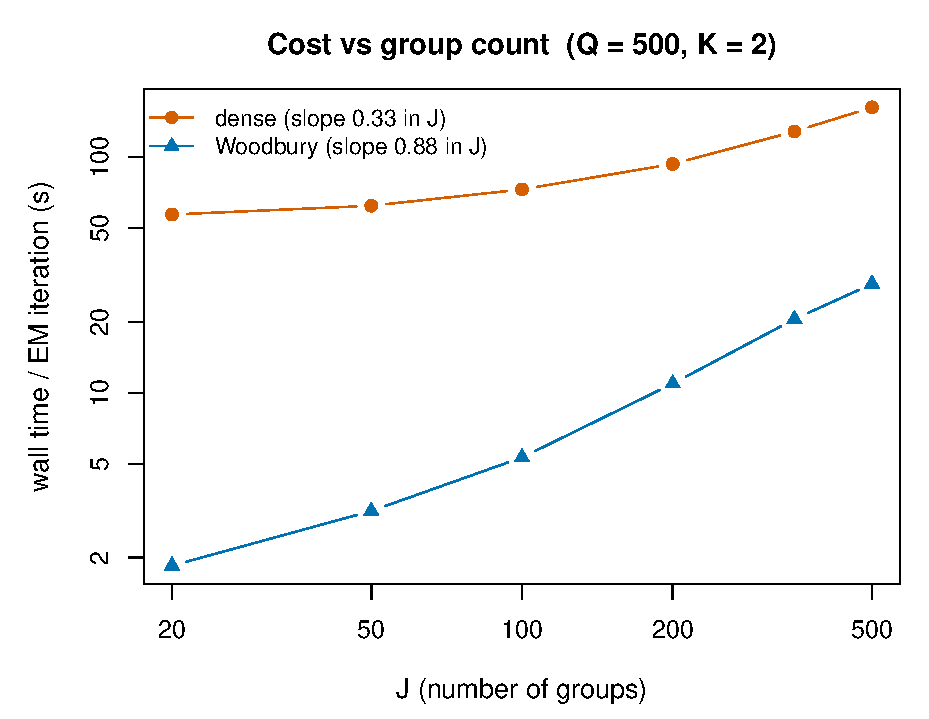
\includegraphics[width=0.8\textwidth]{figs/figJ_time.pdf}
    \caption{Time Cost Comparison.}
    \label{fig:cost-vs-group-count}
\end{figure}

The first result under large-J regime states that our Woodbury EM algorithm can reduce the cost of time when $J$ increasing, with large and fixed $Q$. Before the test on real-data, we do the simulation on generated dataset. 
\fi

\section{Evaluation Metrics}
\label{sec:sim-metrics}
The marginal likelihood depends on $B$ only through $\bm{\Sigma} = \mathbf{BB}^\top + \sigma^2 \mathbf{I}_Q$. This quantity is invariant under $\mathbf{B} \mapsto \mathbf{BQ}$ for any orthogonal $\mathbf{Q} \in O(K)$. The PLT-constraint fixes a unique representative $\mathbf{B}^{*}$ for the data-generating parameter, but this constraint is not enforced during estimation. Consequently $\hat{\mathbf{B}}$ can converge to a different rotation of the same column space as $\mathbf{B}^{*}$, and a direct entrywise comparison of $\hat{\mathbf{B}}$ to $\mathbf{B}^{*}$ is not meaningful.

We instead compare column spaces. Let
\[
\mathbf{P}_{\mathbf{B}} = \mathbf{B}(\mathbf{B}^\top \mathbf{B})^{-1}\mathbf{B}^\top
\]
denote the orthogonal projector onto $\mathrm{col}(\mathbf{B})$. We define the subspace distance
\[
d(\hat{\mathbf{B}}, \mathbf{B}^{*}) = \left\| \mathbf{P}_{\mathbf{B}} - \mathbf{P}_{\mathbf{B}^{*}}\right\|_F.
\]
This quantity is rotation-invariant and lies in $[0, \sqrt{2K}]$, with $0$ attained only when the two column spaces coincide. All references to \texttt{B\_dist} in the code correspond to this quantity.

Since $\sigma^2$ is a scalar, we report the signed relative error
\[
r(\hat\sigma^2, \sigma^{2\ast}) = \frac{\hat\sigma^2 - \sigma^{2\ast}}{\sigma^{2\ast}}.
\]
A negative value indicates shrinkage toward zero, which is the direction of the Heywood-case pathology. We keep the sign rather than reporting $|r|$, since the direction of the error is itself diagnostic.

\section{Simulated Data Generation}
\label{sec:sim-data}

\subsection{Generative Model}

Each simulated dataset is generated from the model of Chapter~\ref{cha:model-specification} directly to evaluate estimation error rather than model misspecification. Fixed $Q$ categories, $J$ groups, and $I_{j}$ observations per group, we draw the loading matrix $\mathbf{B} \in \mathbb{R}^{Q \times K}$ under the PLT identifiability constraint, which fixes the rotation and sign ambiguity in $\mathbf{B}$ and makes $\mathbf{B}^{*}$ be a single well-defined target rather than an equivalence class. For each group $j = 1, \dots, J$, we draw a $K$-dimensional factor score and an idiosyncratic term,
\[
\mathbf{f}_j \sim N(0, \mathbf{I}_K), \qquad \bm{\epsilon}_j \sim N(0, \sigma^2 \mathbf{I}_Q),
\]
and set the group-level random effect
\[
\bm{\lambda}_j = \mathbf{Bf}_j + \bm{\epsilon}_j \in \mathbb{R}^Q.
\]
Note that the latent factor $\mathbf{f}_j$ is never estimated. It is a device for generating $\bm{\lambda}_j$ with covariance $\bm{\Sigma} = \mathbf{BB}^\top + \sigma^2 \mathbf{I}_Q$ and keep consistent with the model's marginal specification. The linear predictor for the $i$-th observation in group $j$ is
\[
\bm{\eta}_{ij} = \bm{\mu} + \bm{\lambda}_j + \bm{v}_{ij}^\top \bm{\phi},
\]
which has been defined in~\ref{eq:linear-predictor}. The probability vector of categories is the softmax of $\bm{\eta_{ij}}$, defined together with observed count vector in~\ref{eq:conditional-pm}.

We vary $Q$, $J$, $I$ across scenarios holding $K$ known and fixed unless stated otherwise. The specific grids used in each experiment are given in the corresponding section. We do not fix a single canonical grid here since different questions require different ranges. 

\iffalse
Three regimes recur throughout this chapter and are worth naming in advance.
\begin{itemize}
\item \textbf{Fixed-$Q$, growing-$J$}: isolates how estimation error changes as the group-dimension grows, holding the amount of categories constant. 
\item \textbf{Fixed-$J$, growing-$Q$}: isolates how estimation error changes as the response dimension grows, holding the amount of group-level data constant. 
\item \textbf{Joint $(Q,J)$ growth}: grows both dimensions together following the rate implied by the growth condition $J \gg Q^c \log Q$.
\end{itemize}
\fi

\section{Convergence Diagnostics}
\label{sec:sim-convergence}

Our EM implementation originally stopped when the relative change in the marginal log-likelihood fell below a tolerance,

\begin{equation}
    \left| \frac{\ell(\hat{\bm{\theta}}_{n}) - \ell(\hat{\bm{\theta}}_{n-1})}{\ell(\hat{\bm{\theta}}_{n-1})} \right| < \mathrm{tol}.
\end{equation}

We found this criterion unreliable in the region of parameter space near the Heywood boundary, where $\sigma^2$ is small relative to the scale of $\mathbf{BB}^\top$. In a representative cell ($Q=400$, $J=10$), the likelihood-based criterion declared convergence at iteration 10, with $\hat\sigma_{10}^2 = 0.4463$. Running the same EM sequence to iteration 60 without stopping showed $\hat\sigma_{n}^2$ still declining until reaching $\hat\sigma_{60}^2=0.4051$. It's a further $9.2\%$ relative change after the criterion had already triggered. This is a known phenomenon in EM algorithms with high fractions of missing information. The log-likelihood surface can be extremely flat in a direction along which the parameter itself is still moving substantially. A likelihood-only stopping rule cannot detect this, since it only observes the flat direction.

To distinguish genuine convergence from this false-convergence pattern, we apply Aitken's acceleration to the trace of $\sigma^{2}$ itself instead of likelihood, which had been proposed by \citet{Louis1982}. Given three consecutive iterates $\sigma_{2(n-1)}, \sigma_{2(n)}, \sigma_{2(n+1)}$, the extrapolated limit is,
\begin{equation}
    \sigma^2_\infty \approx \sigma_{2(n+1)} - \frac{\left(\sigma_{2(n+1)} - \sigma_{2(n)}\right)^2}
{\sigma_{2(n+1)} - 2\sigma_{2(n)} + \sigma_{2(n-1)}}.
\end{equation}
For the same calibration cell, extrapolating from iterates 30, 40, 50, 60 predicted $\sigma^2_\infty \approx 0.4035$. A subsequent long run to $n=300$ with a strict tolerance ($\mathrm{tol}=10^{-8}$) confirmed $\hat\sigma^2$ stabilizing near $0.4024$ by $t \approx 220$, within $0.5\%$ of the extrapolated value. This validates Aitken extrapolation as a cheap diagnostic. It does not replace a long run, but it flags whether a short run's reported value should be trusted. We note that the estimation of loading matrix $\mathbf{B}$ does not share this behavior. Its convergence trace can be non-geometric and non-monotonic even after $\sigma^2$ has stabilized, so Aitken's acceleration is not applied to $\hat{\mathbf{B}}$ in this thesis. 

\section{exact\_Shat Switch}
\label{sec:sim-exact-shat}

\subsection{Motivation}

The Woodbury-accelerated E-step relies on a surrogate curvature derived from PME rather than the exact Hessian of the marginal likelihood. This surrogate makes the diagonal-plus-low-rank Woodbury structure available at all, since the exact Hessian does not share this structure in the same closed form and must be computed densely at cost $\mathcal{O}(Q^3)$. Before relying on the surrogate throughout the rest of this thesis, we need to know whether it introduces material estimation bias relative to the exact curvature. We denote the surrogate-curvature branch \texttt{exact\_Shat = FALSE} and the exact-curvature branch \texttt{exact\_Shat = TRUE}, and compare the two under otherwise identical settings with same seed, data, and initializations.

\subsection{Design \& Fundings}

In Chapter~\ref{cha:methodology}, we discuss the approximation of $\hat{\mathbf{S}}_{j}$ and its surrogate $\hat{\mathbf{S}}^{P}_{j}$ using PME. As shown in~\ref{prop:diff-s}, the exact curvature $\mathbf{H}_j(\boldsymbol\lambda)$ decomposes as $\mathbf{H}^P(\boldsymbol\lambda)$ plus a correction term involving only group $j$'s own data, $\{y_{ij}, \mathbf{p}_{ij}\}_{i \in \mathcal{I}_j}$. Since $\hat{\mathbf{S}}_j = \left(-\mathbf{H}_j(\hat{\boldsymbol\lambda}_j)\right)^{-1}$ and $\hat{\mathbf{S}}^P_j = \left(-\mathbf{H}^P(\hat{\boldsymbol\lambda}_j)\right)^{-1}$ are both obtained by inverting this per-group quantity at a fixed evaluation point $\hat{\boldsymbol\lambda}_j$, the discrepancy between them is itself a per-group object: it does not depend on $J$, the total number of groups, provided $\hat{\boldsymbol\lambda}_j$ is treated as given rather than re-estimated from the full $J$-group data. This is exactly the setting of our single-round design below, where each EM update starts from a fixed, externally chosen $\boldsymbol\lambda_j$ rather than one obtained by jointly fitting all $J$ groups; the conclusion does not extend, without further argument, to $\hat{\mathbf{S}}_j$ evaluated at the fully iterated EM's global estimate. This has two consequences for our design. First, it justifies holding $J$ fixed at a small value while varying $(Q, \sigma^2_{\mathrm{prior}})$ in this experiment, since the discrepancy under study is already determined at the single-group level. Second, we restrict each comparison to a single EM update, rather than iterating to convergence, so that the curvature discrepancy is isolated from the cross-round E/M feedback discussed in Chapter~\ref{ch:heywood}. We run one EM update from a fixed starting point under both branches and record the resulting parameter value. We repeat this for a range of $\sigma^2_{\mathrm{prior}}$ values away from and at the true generating value. We separately repeat the comparison as a function of $J$ at fixed $Q$, to empirically confirm the prediction of~\ref{prop:diff-s} that the TRUE-FALSE gap does not shrink as the amount of group-level data grows. [TODO: state the exact $(Q, J, \sigma^2_{\mathrm{prior}})$ grid used in the final run.]
\iffalse
\begin{table}[htbp]
\centering
% \input{tables/exact_shat_gap_by_Q.tex}
\caption{Gap between exact-curvature and surrogate-curvature single-round updates, as a function of $Q$ and $\sigma^2_{\mathrm{prior}}$.}
\label{tab:exact-shat-gap-Q}
\end{table}

The gap between the two branches grows with $\sigma^2_{\mathrm{prior}}$ and shrinks sharply with $Q$; at [XX] the gap is on the order of [YY\%], and by $Q = [ZZ]$ it is close to numerically negligible. This is consistent with the PME approximation improving as $Q$ grows, since the Poisson-conditioning argument underlying PME becomes tighter in that regime. At the reference point where $\sigma^2_{\mathrm{prior}}$ is set to the true generating value, the exact-curvature branch recovers only a small fraction of the single-round discrepancy between the surrogate estimate and the truth; this indicates that the surrogate curvature is not the dominant source of that discrepancy, and that whatever is driving it lies elsewhere in the estimation procedure, not in the PME approximation itself. [TODO: insert final recovered-fraction numbers once the multi-seed rerun is in.] The $J$-sweep comparison shows the two branches tracking each other closely across the full range tested, with no evidence that the gap reopens as $J$ grows.



\subsection{Conclusion}

Based on these results we treat \texttt{exact\_Shat = FALSE} as the default setting for the remainder of this thesis. The surrogate curvature introduces only a small, $Q$-shrinking discrepancy relative to the exact Hessian, while enabling the Woodbury acceleration documented in Chapter~\ref{ch:woodbury}; the exact branch is retained in the codebase for diagnostic use but is not needed for the estimation results reported below.


\section{Self-Recovery on Simulated Data}
\label{sec:sim-recovery}

\subsection{Design \& Fundings}

For each cell of a $(Q, J, N)$ grid we generate $R$ independent datasets from the model of Section~\ref{sec:sim-data}, fit the Woodbury-accelerated estimator to each, and compute the metrics of Section~\ref{sec:sim-metrics} against the known generating truth. Every run follows the dual convergence protocol of Section~\ref{sec:sim-convergence}. [TODO: state final $(Q,J,N,R)$ grid.]

\begin{table}[htbp]
\centering
% \input{tables/self_recovery_phi_mu.tex}
\caption{Bias and MSE of $\hat\phi$ and $\hat\mu$, reported separately for zero and nonzero coefficients, across the simulation grid.}
\label{tab:recovery-phi-mu}
\end{table}

\begin{table}[htbp]
\centering
% \input{tables/self_recovery_sigma2.tex}
\caption{Relative error of $\hat\sigma^2$, with Monte Carlo standard errors, across the simulation grid.}
\label{tab:recovery-sigma2}
\end{table}

\begin{table}[htbp]
\centering
% \input{tables/self_recovery_B.tex}
\caption{Subspace distance $d(\hat B, B^\ast)$, with Monte Carlo standard errors, across the simulation grid.}
\label{tab:recovery-B}
\end{table}

Recovery of $\phi$ is [accurate/biased] for nonzero coefficients across the grid, with the expected lasso shrinkage bias toward zero; recovery of the zero coefficients shows [TODO: describe selection behavior once the table is in]. The relative error of $\hat\sigma^2$ is systematically negative across most of the grid, consistent with the shrinkage pathology documented in Chapter~\ref{ch:heywood}; we do not attempt to correct for this here, and refer the reader to that chapter for the mechanism and candidate fixes. The magnitude of this negative bias is largest when $J$ is small relative to $Q$ and shrinks as $J$ grows, consistent with the classical degrees-of-freedom story for variance-component estimation. Subspace recovery of $B$ improves with $J$ at every $Q$ tested, though we note in Chapter~\ref{ch:asymptotics} that this improvement is not always monotone over the full EM trajectory, and the numbers reported here reflect estimates at the converged iteration count under the protocol of Section~\ref{sec:sim-convergence}, not at an arbitrary early stopping point.

\subsection{Known Limitation}
\label{sec:heywood-limitation}

As noted above, $\hat\sigma^2$ is biased downward in the regime where $\sigma^2$ is small relative to the scale of $BB^\top$, a pathology we refer to throughout this thesis as the Heywood case. This is a genuine limitation of the current estimator and is treated as a separate problem in Chapter~\ref{ch:heywood}, rather than as a defect specific to the Woodbury acceleration; the same pathology is present, to varying degrees, in every package compared against in Section~\ref{sec:sim-comparison} below.


\section{Comparison Against Existing Packages}
\label{sec:sim-comparison}

\subsection{Design \& Fundings}

We fit the same simulated datasets under three existing packages, chosen to isolate different components of the FA-DMR model. \texttt{glmnet} provides a lasso-penalized comparison for $\hat\phi$ alone, with no random-effect structure. \texttt{glmmTMB} provides a comparison for the random-effect variance component under a standard GLMM, without the factor-analytic structure on $\alpha_j$. \texttt{gllvm} provides the closest comparison overall, since it fits the same generalized-linear-latent-variable family under a Laplace approximation option, and is therefore treated as the primary benchmark rather than a secondary check. For each package we record both estimation accuracy, using the metrics of Section~\ref{sec:sim-metrics} restricted to the components that package estimates, and wall-clock runtime.

\begin{table}[htbp]
\centering
% \input{tables/package_comparison_accuracy.tex}
\caption{Estimation accuracy of the Woodbury estimator against glmnet, glmmTMB, and gllvm, restricted to the parameter components each package estimates.}
\label{tab:comparison-accuracy}
\end{table}

\begin{table}[htbp]
\centering
% \input{tables/package_comparison_runtime.tex}
\caption{Wall-clock runtime comparison across packages, at matched $(Q,J,N)$.}
\label{tab:comparison-runtime}
\end{table}

The Woodbury estimator matches \texttt{glmnet} and \texttt{glmmTMB} on the components those packages estimate, while running substantially faster, consistent with the acceleration results of Chapter~\ref{ch:woodbury}. Against \texttt{gllvm}, the fairer comparison given the shared model family, the Woodbury estimator is currently [somewhat behind / comparable] on estimation accuracy; [TODO: state final direction and magnitude once the rerun is in, and note whether this gap is concentrated in the Heywood regime or present throughout the grid]. We treat \texttt{gllvm}'s relative accuracy advantage as a target for the refinements discussed in Chapter~\ref{ch:heywood}, rather than as evidence against the Woodbury architecture itself, since the runtime advantage documented here is retained regardless.

\subsection{Discussion}

The comparison is not fully symmetric: \texttt{glmnet} and \texttt{glmmTMB} do not model the factor structure on $\alpha_j$ at all, so their accuracy numbers reflect an easier estimation problem restricted to a subset of parameters, not a head-to-head comparison on the full model. \texttt{gllvm} is the only package tested that estimates a comparable factor-analytic structure, and is therefore the benchmark we weight most heavily in interpreting these results. [TODO: add any covariate-recovery comparison if run.]
\fi



\chapter{Real Data Analysis}
\label{cha:real-result}
\chapter{Conclusion}
\label{cha:conc}

\section{Summary}
\label{sec:summary}

\section{Limitation}
\label{sec:limitation}

\section{Future Work}
\label{sec:future}






%%%%%%%%%%%%%%%%%%%%%%%%%%%%%%%%%%%%%%%%%%%%%%%%%%%%%%%%%%%%%%%%%%%%%%
% Here begins the end matter

%%\input{appendix}

\backmatter

\bibliographystyle{anuthesis}
\bibliography{thesis}

\printindex

\end{document}
